\documentclass[12pt,a4paper,openright,oneside]{book}
\usepackage[utf8]{inputenc}

\newcommand{\thesislang}{italian} % decommentare in caso di tesi in italiano
%\newcommand{\thesislang}{english} % commentare in caso di tesi in italiano
\usepackage{thesis-style}

\begin{document}

\frontmatter

\title{Title}
\author{Enrico Siboni}
\date{01/12/2019}

\newgeometry{margin=0.8in}
\begin{titlepage}
	\begin{center}
		% \vspace*{0.2cm}
		
		\large
		\textbf{ALMA MATER STUDIORUM -- UNIVERSITÀ DI BOLOGNA \\ CAMPUS DI CESENA}
		\\
		\noindent\hrulefill
		\vspace{0.4cm}
		
		\Large
		Scuola di Scienze \\
		Corso di Laurea in Ingegneria e Scienze Informatiche
		
		%\Huge
		\vspace{4cm}
		\begin{center}
        {\large{\bf PROGETTAZIONE E IMPLEMENTAZIONE DI AGENTI}}\\
        \vspace{2mm}
        {\large{\bf CON CAPACITÀ DI NAVIGAZIONE COGNITIVA PER}}\\
        \vspace{2mm}
        {\large{\bf SIMULAZIONI DI EVACUAZIONI DI FOLLE IN ALCHEMIST}}\\
        \end{center}
		
		\large
		\vspace{1cm}
		Tesi di laurea in 
		\\
		\textsc{Programmazione ad oggetti}
		
		\vspace{5.5cm}
		\begin{minipage}[t]{0.64\textwidth}
			\begin{flushleft}
				\textit{Relatore} 
				\\ 
				\textbf{Prof.} \textbf{Mirko Viroli}
				\\
				\vspace{0.4cm}
				\textit{Correlatore} 
				\\
				\textbf{Prof.} \textbf{Danilo Pianini}
			\end{flushleft}
		\end{minipage}
		\begin{minipage}[t]{0.34\textwidth}
			\begin{flushright}
				\textit{Candidato} 
				\\ 
				\textbf{Lorenzo Paganelli}
			\end{flushright}
		\end{minipage}\\
		
		\vfill
		\noindent\hrulefill
		\vspace{0.3cm}
		\Large
		
		Terza Sessione di Laurea
		\\
		Anno Accademico 2018-2019
	\end{center}
\end{titlepage}
\restoregeometry

\begin{abstract}	
La simulazione computerizzata di folle in movimento è stato un campo piuttosto attivo recentemente, con applicazioni che vanno dall’intrattenimento alla gestione della sicurezza in luoghi pubblici o privati. Le simulazioni di folle devono prendere in considerazione non solo gli aspetti fisici dell’ambiente e dei pedoni, ma anche i fattori psicologici e sociali che hanno un effetto sul movimento delle persone. La capacità di orientarsi all’interno di un ambiente è una caratteristica fondamentale dell'essere umano e in quanto tale è indispensabile per una simulazione realistica. Diversi modelli assumono che i pedoni abbiano conoscenza totale dell’ambiente, cioè che ne conoscano la topologia e le metriche per intero. Ciò può essere ammissibile quando il processo di navigazione è triviale, ad esempio in una piazza, tuttavia in ambienti più complessi questa è una grezza approssimazione, in quanto difficilmente ciascun pedone ne possiede una conoscenza completa (specie se molte delle persone coinvolte visitano l’edificio per la prima volta). Lo scopo del lavoro corrente è modellare la rappresentazione mentale che ciascun pedone ha dell’ambiente circostante, spesso parziale e inaccurata, e il processo mentale in atto in ogni persona che usa tali informazioni per scegliere quale percorso o direzione seguire (cioè orientarsi); i modelli sono poi implementati all’interno del simulatore Alchemist adottando un approccio ad agenti. 

Di particolare interesse per il lavoro corrente sono le simulazioni di evacuazioni di folle, per il loro valore nel prevenire situazioni disastrose durante la pianificazione di eventi o la progettazione di edifici. Detto ciò, i modelli presentati sono pensati per essere usati in qualsiasi tipo di simulazione.
\end{abstract}

%\begin{dedication} % this is optional
%Optional. Max a few lines.
%\end{dedication}

%\begin{acknowledgements} % this is optional
%Optional. Max 1 page.
%\end{acknowledgements}

%----------------------------------------------------------------------------------------
\tableofcontents   
%\listoffigures     % (optional) comment if empty
%\lstlistoflistings % (optional) comment if empty
%----------------------------------------------------------------------------------------

\mainmatter

%----------------------------------------------------------------------------------------
\chapter{Contesto e motivazioni}
\label{chap:background}
%----------------------------------------------------------------------------------------

\section{L'evacuazione di folle}
Al giorno d’oggi, le occasioni in cui un grande numero di persone si raduna in uno spazio relativamente ristretto sono piuttosto frequenti, si pensi ad esempio alla quantità di eventi su larga scala legati allo sport, l’intrattenimento, la cultura o la religione che prendono luogo regolarmente. In queste situazioni la sicurezza è un aspetto centrale ed è necessario essere preparati per ogni tipo di criticità. Solitamente, in situazioni d’emergenza i partecipanti devono essere condotti lontano dalla zona di pericolo o presunto tale nel minor tempo possibile. Talvolta, però, l’evacuazione può sfociare in una fuga incontrollata che muta l’evento in tragedia, come dimostrano gli eventi di piazza San Carlo a Torino (che comunque costituiscono solo uno dei molteplici esempi della pericolosità legata alle evacuazioni), si veda la \cref{fig:piazza-san-carlo}. Per evitare situazioni di pericolo, gli organizzatori seguono protocolli di sicurezza ed effettuano simulazioni di evacuazione in vari scenari. Tuttavia, un difetto non trascurabile delle simulazioni reali è la radicale differenza delle condizioni psicologiche dei partecipanti rispetto ad una situazione di vero o presunto pericolo. In più, i costi possono essere proibitivi: una simulazione organizzata dalla UK Marine Coastguard Agency sul traghetto “Stena Invicta” tenutasi al porto di Dover nel 1996 costò più di 10,000 GPB \cite{MSAEvacuationSimulation}. In questo senso, le simulazioni computerizzate possono talvolta costituire un’alternativa migliore.
\begin{figure}
	\centering
	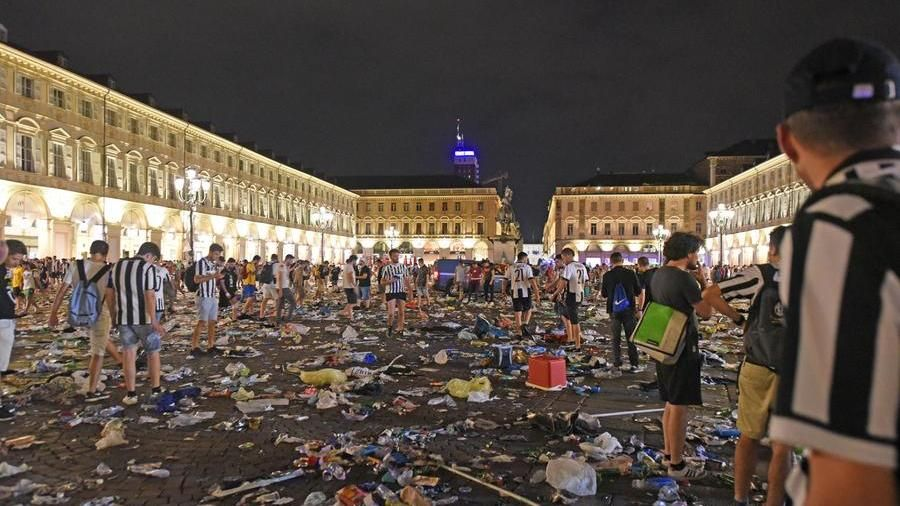
\includegraphics[width=0.8\linewidth]{figures/piazza-san-carlo.jpeg}
	\caption{Piazza San Carlo a Torino poco dopo la fuga incontrollata della folla, scaturita dal panico e dalla calca causati dall'utilizzo di spray urticante da parte di malviventi, che ha causato più di 1500 feriti nonché la morte di tre persone.}
	\label{fig:piazza-san-carlo}
\end{figure}

\section{La simulazione computerizzata}
La simulazione computerizzata, rispetto a quella reale, presenta costi assai più ridotti e generalmente è in grado di valutare più scenari in minor tempo. In letteratura esistono diversi tipi di modelli per la simulazione di folle in movimento, ciascuno differisce per una gamma di caratterestiche descritte di seguito. Obbiettivo comune di tali modelli, però, è quello di riprodurre comportamenti realistici della folla, ossia comportamenti osservati empiricamente. I diversi modelli possono essere classificati sulla base delle seguenti caratteristiche \cite{SchadschneiderEvacuationDynamics2009}:
\begin{itemize}
 \item \textbf{Granularità}: Per quanto riguarda la granularità della folla, i modelli vengono divisi in microscopici e macroscopici. Nei modelli microscopici ciascun individuo è rappresentato separatamente, solitamente permettendo di avere eterogeneità tra questi. In contrasto, nei modelli macroscopici è impossibile distinguere i singoli individui: ad esempio i modelli fluidodinamici rappresentano la folla nella sua interezza come, appunto, un fluido.
 \item \textbf{Spazio e tempo}: Per descrivere un sistema di pedoni in movimento si usano variabili che descrivono il tempo, lo spazio e lo stato (e.g. velocità dei pedoni). Ciascuna di queste variabili può essere discreta (i.e. un numero intero) o continua (i.e. un numero reale), ogni combinazione è possibile. I modelli basati su automi cellulari, ad esempio, descrivono lo spazio in maniera discreta.
 \item \textbf{Casualità}: I modelli possono essere distinti in deterministici e stocastici. Nei modelli deterministici il comportamento di un pedone in un certo istante è completamente determinato dal suo stato attuale, non c'è casualità. Nei modelli stocastici, invece, il comportamento degli individui è influenzato da un grado di casualità, in modo che un individuo possa reagire in maniera differente alla stessa situazione. Inoltre, l'introduzione di casualità nel modello può talvolta riflettere la mancanza di conoscenza riguardo i reali processi fisici o mentali in atto nei pedoni.
 \item \textbf{Interazione tra i pedoni}: Per quanto riguarda l'interazione tra gli individui, vengono solitamente distinti modelli basati su regole (o rule-based) e modelli basati su forze (o force-based). Nei primi, i pedoni prendono decisioni sulla base del proprio stato e dell'ambiente circostante, le regole che ne descrivono il comportamento sono spesso derivate dalla psicologia. Nei modelli force-based, invece, i pedoni subiscono forze suscitate dall'ambiente o dagli individui circostanti. Tali forze modellano comportamenti osservati empiricamente, come ad esempio la tendenza ad evitare agglomerati di persone, o ad aggirare ostacoli in un certo modo. 
 In questo caso, una netta distinzione tra i due tipi di interazione non è sempre possibile e diversi modelli combinano elementi di entrambi gli approcci.
\end{itemize}

Di particolare interesse per il lavoro corrente sono i modelli ad agenti e i modelli basati su forze sociali, entrambi categorizzabili come approcci microspici, ma differenti per il tipo di interazione tra i pedoni.
\paragraph{Modelli ad agenti.} I modelli basati sugli agenti approssimano il sistema ad un insieme di entità capaci di interagire tra loro e di prendere delle decisioni autonome basate su un insieme di regole. Ciascun agente percepisce ciò che accade nell’ambiente circostante, prende una decisione sulla base di questo e del suo stato interno, infine agisce. Tali modelli simulano le azioni locali di ciascun pedone e permettono di avere eterogeneità tra questi, essendo che ognuno è dotato di un proprio stato interno mutabile che lo rende diverso dagli altri. L’eterogeneità è essenziale per la realizzazione di pedoni con diversi gradi di conoscenza dell’ambiente. 
\paragraph{Modelli basati su froze sociali.} I modelli basati sulle forze sociali \cite{HelbingSocialForce1998} considerano il movimento dei pedoni come la somma di diversi stimoli, ad esempio la volontà di raggiungere una destinazione o di mantenere una certa distanza da eventuali ostacoli. La combinazione di questi stimoli, chiamati appunto forze sociali, determina la velocità e la direzione del movimento di un pedone in ogni istante. Le forze sociali sono in grado di far emergere comportamenti piuttosto realistici partendo dalla somma di forze più semplici.

\section{Il simulatore Alchemist}
Alchemist \cite{alchemist-jos2013} è un simulatore stocastico nato all’interno dell’Università di Bologna, che permette la simulazione di scenari inerenti la computazione pervasiva, aggregata ed ispirata alla natura. La chiave della pluralità di Alchemist sta nel suo metamodello, descritto di seguito. Qualunque evento rappresentabile mediante tale metamodello può essere simulato via Alchemist. Questa breve introduzione al simulatore ha come scopo quello di far familiarizzare il lettore con le entità costituenti il metamodello, in quanto in fase di progettazione si dovranno rappresentare i concetti introdotti nel \cref{chap:development} per mezzo di tali entità. Per una più completa descrizione di Alchemist si veda il sito ufficiale\footnote{\url{https://alchemistsimulator.github.io}}.

\subsection{Il metamodello di Alchemist}
Le entità costituenti il metamodello di Alchemist sono le seguenti:
\begin{itemize}
 \item \textbf{Molecola}: corrispettivo del concetto di variabile in un linguaggio di programmazione.
 \item \textbf{Concentrazione}: valore associato a una particolare molecola.
 \item \textbf{Nodo}: contenitore di molecole e reazioni, posizionato all’interno di un ambiente.
 \item \textbf{Ambiente}: contenitore di nodi, modella il concetto di spazio.
 \item \textbf{Reazione}: evento che può modificare l’ambiente, è costituito da condizioni e azioni. Ogni nodo ha un insieme di reazioni che ne definiscono il comportamento.
 \item \textbf{Condizione}: funzione booleana che determina se la reazione associata deve essere eseguita.
 \item \textbf{Azione}: modella un qualunque cambiamento dell’ambiente 
\end{itemize}
La \cref{fig:alchemist-meta-model} dà una rappresentazione grafica di tali entità. 
\begin{figure}
	\centering
	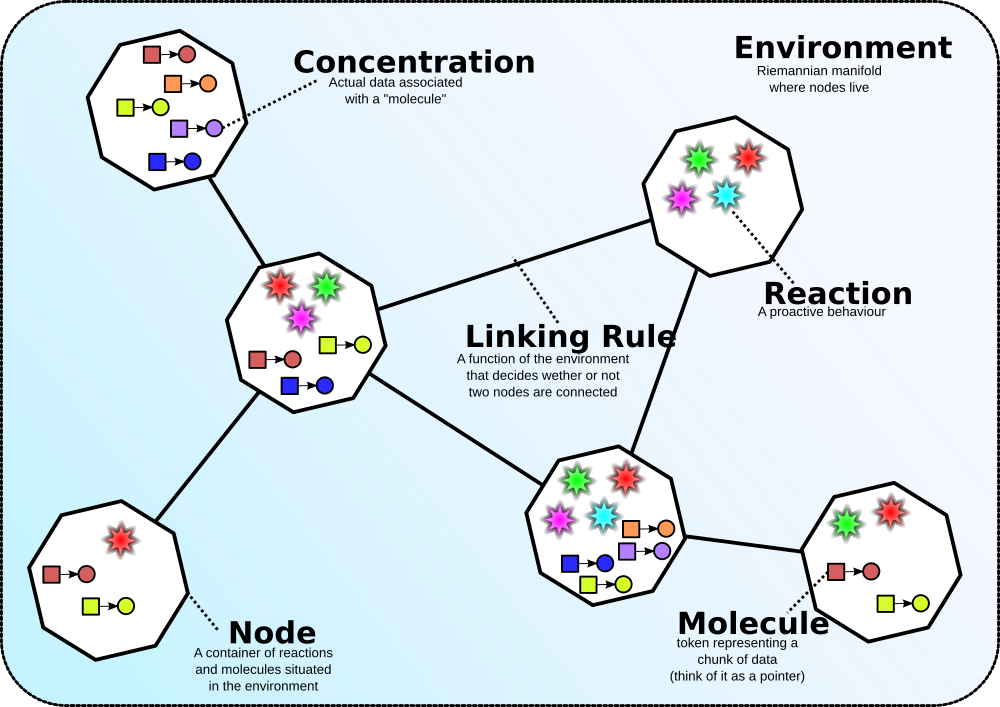
\includegraphics[width=0.8\linewidth]{figures/alchemist-meta-model.png}
	\caption{Il metamodello di Alchemist.}
	\label{fig:alchemist-meta-model}
\end{figure}
Queste sono ispirate al mondo della chimica perlopiù per ragioni storiche, nonostante questo il simulatore è in grado di modellare gli eventi più vari. La natura della sua generalità sta nell’ampia interpretazione dei concetti di molecola e concentrazione: questi due termini hanno un significato ben preciso in chimica, ma in Alchemist corrispondono rispettivamente ad un identificatore e un dato di qualche tipo.

\subsection{L'evacuazione di folle in Alchemist}
Alchemist è dotato delle astrazioni necessarie a simulare l'evacuazione di folle i cui pedoni presentano diverse caratteristiche fisiche (come sesso ed età), psicologiche (come paura e sensazione di pericolo) e sociali (come la tendenza a rimanere vicino al proprio gruppo sociale). L'approccio adottato è un ibrido basato sul modello ad agenti (che in una certa misura è connaturato al metamodello stesso di Alchemist) con elementi di forze sociali. In particolare, i modelli adottati per descrivere i pedoni sono due: il Network Oriented Modeling \cite{TreurNetworkOrientedModeling2018} viene usato per rappresentare la sfera emotiva di ciascun individuo e la sua evoluzione. Fondamentalmente, tale approccio consiste nell'uso di un grafo orientato per definire processi emotivi interconnessi tra loro. I movimenti della folla, invece, sono realizzati impiegando i comportamenti di steering introdotti da C. W. Reynolds \cite{ReynoldsSteering2002}. Questi descrivono il movimento di un individuo come la somma di diversi stimoli (ad esempio la volontà di rimanere vicino alla propria alla famiglia, la tendenza ad allontanarsi dalle zone di pericolo), e sono dunque classificabili come forze sociali. Tale approccio è in grado di rappresentare il conflitto di interessi in atto in ogni pedone in una situazione di emergenza e pertanto è capace di far emergere comportamenti assai realistici. 

Alla luce di quanto detto finora, si può procedere a classificare Alchemist secondo le quattro caratteristiche descritte in 1.2: esso è un simulatore stocastico che modella spazio, tempo e stato con variabili continue (generalmente più fedeli alla realtà). Ciascun individuo è rappresentato separatamente e c'è eterogeneità tra questi, dunque la granularità è microscopica; infine le interazioni presentano elementi sia degli approcci rule-based che force-based.

I pedoni simulati in Alchemist sono relativamente sofisticati, ma ad ora sprovvisti della capacità di orientarsi all'interno di un ambiente. Scopo del lavoro corrente è fornirli di questa caratteristica, modellando l'inaccuratezza delle informazioni spaziali in possesso di ciascun individuo e il processo mentale che sfrutta queste informazioni ai fini dell'orientamento.

\subsection{Utilizzo}
Il linguaggio utilizzato per la scrittura di simulazioni per Alchemist è YAML\footnote{\url{https://yaml.org}}, un formato per la serializzazione di dati facilmente leggibile dall'uomo. I file di simulazione sono mappe YAML, le principali chiavi utilizzabili sono le seguenti:
\begin{itemize}
    \item \texttt{incarnation}: un'incarnazione è un'istanza del metamodello di Alchemist che definisce il tipo di concentrazione. Al momento esistono quattro incarnazioni, non si entra nei dettagli in quanto non utili ai fini del lavoro corrente. Si sappia unicamente che questa chiave deve indicare quale di queste quattro incarnazioni usare, è l'unica chiave obbligatoria.
    \item \texttt{seeds}: specifica i semi da utilizzare per la generazione di numeri casuali. In particolare, deve essere esplicitato il seme da utilizzare sia durante la creazione che durante l'esecuzione della simulazione. Questi prendono il nome rispettivamente di \texttt{scenario} e \texttt{simulation}.
    \item \texttt{variables}: valori che si vogliono riutilizzare all’interno del file di simulazione, possono essere sia semplici numeri che oggetti complessi.
    \item \texttt{environment}: l'ambiente dentro il quale si svolge la simulazione.
    \item \texttt{displacements}: le posizioni iniziali dei nodi.
\end{itemize}
Per una descrizione più dettagliata delle chiavi utilizzabili si faccia riferimento al sito di Alchemist\footnote{\url{https://alchemistsimulator.github.io/wiki/usage/yaml/}}. Questa breve digressione riguardo l'utilizzo del simulatore ha l'obbiettivo di far familiarizzare il lettore con la modalità di scrittura delle simulazioni, che verrà citata a più riprese nel seguito.

\subsection{Accorgimenti}
Nonostante Alchemist sia un simulatore stocastico, fa della riproducibilità un aspetto essenziale. Al fine di garantirla, è necessario sapere che non è possibile utilizzare un generatore di numeri pseudo-casuali diverso da quello di cui è provvista la simulazione. Inoltre, non è possibile utilizzare strutture dati come \texttt{Set} in cui l'ordine degli elementi non è prederminato. 

%----------------------------------------------------------------------------------------
\chapter{Navigazione cognitiva in Alchemist}
\label{chap:development}
%----------------------------------------------------------------------------------------

\section{Analisi del dominio}
In questa sezione sono presentati i risultati di alcuni studi precedenti inerenti la capacità dell’essere umano di orientarsi all’interno di un ambiente, da questi risultati vengono poi ricavati dei modelli per rappresentare la conoscenza spaziale dei pedoni utilizzabili in simulazioni ad alto numero di agenti. Si noti che tali modelli non sono che un’approssimazione delle reali capacità dell’essere umano di orientarsi e navigare un ambiente, in quanto diversi dei processi mentali coinvolti in questi compiti rimangono tutt’ora sconosciuti.

Prima di procedere è opportuno fare una disambiguazione: in letteratura con il termine “navigazione umana” ci si riferisce a due capacità dell’uomo: la locomozione e l’orientamento. A grandi linee, la locomozione corrisponde all’abilità di muoversi fisicamente, mentre l’orientamento consiste nello scegliere un percorso o una direzione da seguire verso una destinazione o alla ricerca di qualcosa. Nel seguito si parlerà di “navigazione umana” riferendosi all’orientamento, in quanto i pedoni simulati in Alchemist sono naturalmente già dotati della capacità di locomozione.

\subsection{La capacità di orientarsi all'interno di un ambiente}
Diverse delle abilità fondamentali della nostra specie (e.g. viaggiare, mercanteggiare, cacciare) si basano sulla capacità di navigare l’ambiente circostante. Anche in un contesto urbano, l’uomo sfrutta la sua abilità di orientarsi all’interno di spazi aperti o chiusi giornalmente. In letteratura ci si riferisce a questa capacità come \emph{human wayfinding}. Nonostante questo, diversi aspetti dello human wayfinding rimangono tuttora sconosciuti: alcuni compiti, come ad esempio spostarsi da casa al luogo di lavoro, vengono elaborati automaticamente all'interno del cervello senza la necessità di pensieri espliciti \cite{MontelloWayfinding2006}. In particolare, la domanda riguardante \emph{come} diverse strategie e meccanismi mentali lavorino insieme ai fini dello human wayfinding non ha ancora trovato risposta.
Prendere in considerazione l’abilità di orientarsi è indispensabile per le simulazioni di pedoni in movimento: è stato infatti dimostrato che in alcuni scenari tale capacità può influenzare significativamente il progredire dell’evacuazione \cite{AndresenWayfinding2016}. In diverse simulazioni i percorsi seguiti dai pedoni vengono predeterminati con algoritmi capaci di trovare il cammino minimo (o quello ottimo secondo un qualche criterio) tra la posizione di ogni individuo e una qualche destinazione, assumendo dunque che i pedoni abbiano una conoscenza completa dell’ambiente. Come già detto, tale assunzione può essere ammissibile quando il processo di navigazione è banale, come in una piazza, ma è una grezza approssimazione in ambienti più complessi, in cui difficilmente i pedoni hanno una conoscenza completa della topologia e delle metriche. Lo scopo del lavoro corrente è fornire ciascun individuo di un grado di conoscenza diverso dello spazio circostante, per fare ciò è necessario analizzare come gli esseri umani memorizzano e rappresentano la conoscenza spaziale.

\subsection{La conoscenza spaziale}
\label{spatial-knowledge}
La capacità di orientarsi all’interno di un ambiente si basa largamente sulla memorizzazione e valutazione di informazioni spaziali. La fonte primaria di tali informazioni è la mappa cognitiva di ciascun individuo, che consiste nella sua rappresentazione mentale dell’ambiente circostante. In questa sezione vengono presentate le principali fonti di informazioni spaziali.

\subsubsection{Mappa cognitiva} 
La mappa cognitiva, \emph{cognitive map} in letteratura, raffigura la rappresentazione mentale di un individuo dell’ambiente circostante, o meglio della sua topologia. La mappa cognitiva include anche informazioni riguardanti porzioni dell’ambiente non immediatamente percepibili, ad esempio stanze di un edificio già visitate ma lontane dalla posizione corrente. Tale mappa è costituita principalmente da oggetti e relazioni spaziali tra questi \cite{Grling1986ReferenceSI, Golledge1999}. Gli oggetti, chiamati \emph{landmark} in letteratura, sono elementi architettonici in un qualche modo salienti che vengono memorizzati a causa della loro unicità o diversità. Un esempio di landmark potrebbe essere una torre particolarmente alta \cite{Golledge1999}, in generale è stato mostrato che circa metà degli elementi architettonici di una città è considerato come landmark da praticamente ogni persona \cite{Golledge1978}. Per quanto riguarda le relazioni spaziali tra landmark, vengono perlopiù memorizzate informazioni riguardo connessioni dirette o indirette (i.e. rappresentabili con una linea spezzata) tra questi \cite{Golledge1999}. L’uomo tende infatti a determinare la propria posizione e quella di nuovi landmark rispetto a quelle di landmark già memorizzati, che fungono da “ancore” \cite{Golledge1999}. Originariamente, Tolman introdusse il termine cognitive map negli anni 30 quando, conducendo esperimenti sui topi, notò che questi erano in grado di trovare la direzione che li conducesse verso una destinazione già visitata. Tolman \cite{TolmanCognitiveMapRats1948} dedusse quindi che i topi hanno la capacità di memorizzare le posizioni relative di luoghi specifici. Successivamente, capacità simili sono state osservate nell’uomo e in altri mammiferi \cite{EkstromCellularNetworks2003, Ekstrom2010}. La mappa cognitiva consente alle persone di determinare la posizione relativa di una destinazione non visibile elaborando le informazioni in essa contenute. In generale, i landmark hanno un ruolo fondamentale nell’orientamento umano: la scelta del percorso da seguire viene spesso effettuata presso di questi; in più, i segmenti costituenti tale percorso di solito iniziano e finiscono in corrispondenza di landmark \cite{Golledge1999}. In molti casi, le mappe cognitive di ambienti poco familiari sono fornite di scarse informazioni, anche dopo più soggiorni in un ambiente la relativa mappa cognitiva può consistere di informazioni incomplete e inesatte \cite{Golledge1999}. La riproduzione delle mappe cognitive sotto forma di disegni abbozzati mostra poche somiglianze con lo spazio fisico corrispondente \cite{Golledge1999}, i disegni suggeriscono che la mappa cognitiva è piuttosto una rappresentazione imprecisa e astratta dell'ambiente percepito \cite{Carlson2010}; si veda la \cref{fig:cognitive-map-drawing}. Gli errori più frequenti riguardano le distanze tra gli oggetti e gli angoli formati dai vari elementi architettonici  \cite{Golledge1999, Ellard2009}. Tuttavia, le informazioni contenute nella mappa cognitiva, anche se non complete ne dettagliate, possono essere sufficienti per affrontare il problema della navigazione in quanto diversi compiti sono risolvibili con l'aiuto delle relazioni topologiche \cite{Ellard2009}. Una  possibile spiegazione per cui tralasciamo diverse informazioni dettagliate e archiviamo solo parti selezionate e informazioni topologiche sull'ambiente potrebbe essere l'efficienza e i requisiti di memoria minori che accompagnano questa strategia \cite{Ellard2009}.
\begin{figure}
	\centering
	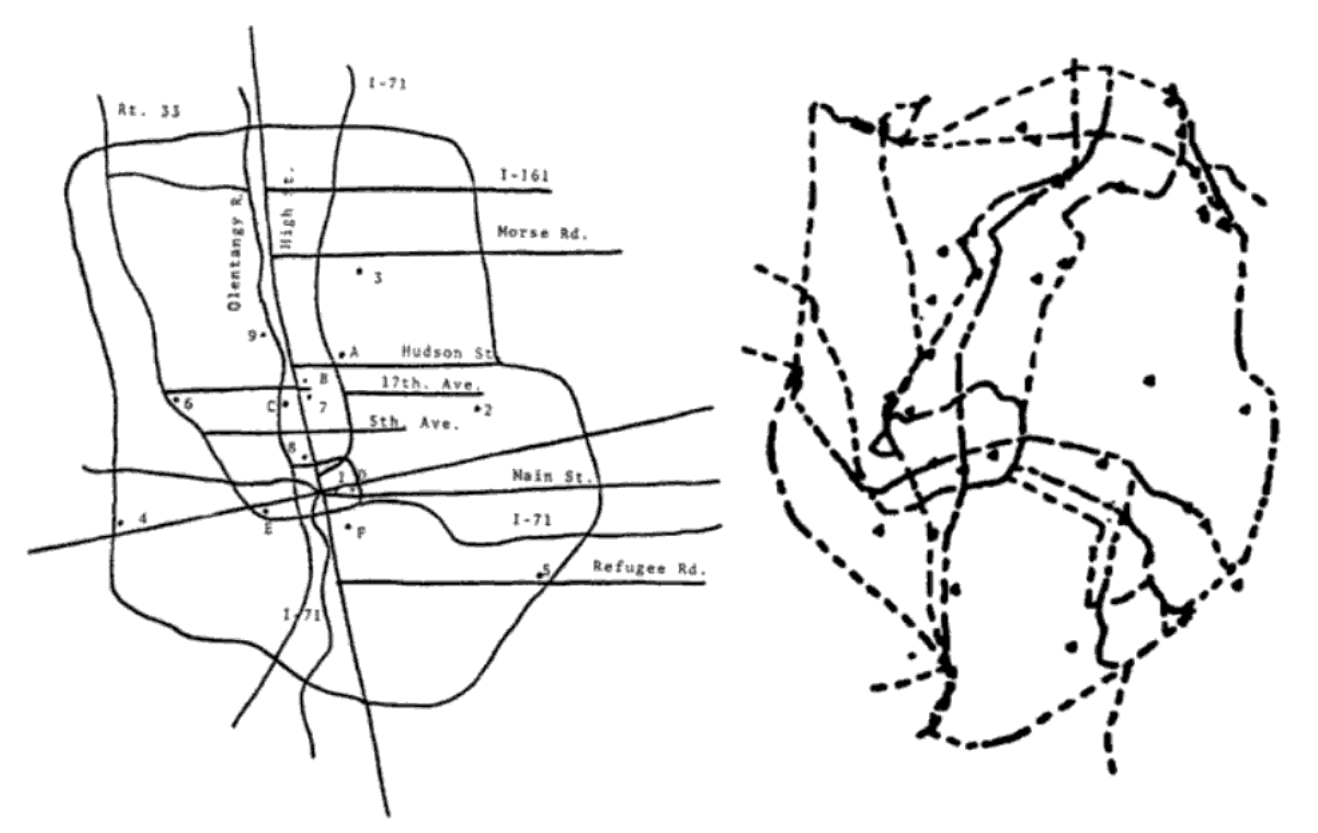
\includegraphics[width=0.8\linewidth]{figures/cognitive-map-drawing.png}
	\caption{A sinistra: mappa reale di Columbus, Ohio. A destra: mappa cognitiva di un residente del posto.}
	\label{fig:cognitive-map-drawing}
\end{figure}


\subsubsection{Conoscenza generalizzata} 
Gli esseri umani tendono a classificare le proprie esperienze: ogni volta che ci si trova in una nuova situazione questa viene prima confrontata con altre simili di cui si è già fatto esperienza, poi categorizzata di conseguenza. Dopodiché, le vengono associati attributi come aspettative e implicazioni relativi alla classe selezionata \cite{Anderson2005, StPierre2014}. Questo processo può essere utile ai fini della navigazione: anche quando un individuo si trova in un ambiente mai visitato prima, infatti, può ricavare informazioni riguardo il tipo di ambiente mediante il processo descritto. Le informazioni non riguardano la topologia dello specifico ambiente, quanto più alcune caratteristiche che spazi di questo tipo condividono \cite{kalff2009, Wiener2009}. Ad esempio, immaginando di trovarsi in una stazione metropolitana (sottosuolo), in una scenario di evacuazione le persone cercherebbero naturalmente una scala per risalire. Questo tipo di conoscenza è chiamata conoscenza generalizzata, in letteratura \emph{generalised knowledge} o \emph{background knowledge}.

\subsubsection{Informazioni esterne} 
Le fonti di informazioni esterne al pedone sono perlopiù due: la segnaletica (quando presente) e gli altri pedoni. Durante le evacuazioni le informazioni provenienti dalle altre persone sono ampiamente sfruttate da coloro che hanno scarsa familiarità con l’ambiente. In particolare, chi non conosce l’ambiente tende a seguire la folla, assumendo che questa ne abbia una conoscenza più estesa e che entrambi abbiano lo stesso obbiettivo: trovare un’uscita (o comunque mettersi in salvo). Questo comportamento è noto come \emph{herding} \cite{Helbing2002}.

\subsection{Il modello di Andresen et al. per lo human wayfinding}
Per poter utilizzare quanto descritto finora in  simulazioni di evacuazioni di folle è necessario ricavare un modello che descriva come questi concetti possano essere usati in un contesto simile. In particolare, è necessario modellare sia la conoscenza spaziale sia il processo di elaborazione di tale conoscenza, di cui finora si è parlato poco. In più, il modello deve essere adatto ad essere usato in simulazioni con un grande numero di agenti. Un approccio che presenta tutte le caratteristiche elencate è quello proposto da Andresen et al. \cite{Andresen2018}, al cui lavoro questa tesi è largamente ispirata. In questa sezione viene descritta una variante di tale modello a cui sono state apportate alcune modifiche per renderlo più adatto alle esigenze del lavoro corrente. Tra le varie fonti di informazioni spaziali descritte in \ref{spatial-knowledge} si è scelto di utilizzare unicamente la mappa cognitiva, in quanto riveste un ruolo privilegiato nello human wayfinding. In futuro, il modello potrà essere esteso con le altre fonti di informazione.

\subsubsection{Rappresentare l'ambiente} 
L’ambiente viene rappresentato con un grafo \(G = (V, E)\) dove i vertici sono poligoni convessi rappresentanti le zone dell’ambiente percorribili dai pedoni, in letteratura \emph{walkable areas}, e gli archi descrivono le connessioni tra le varie zone. Per rendere più chiara questa rappresentazione si pensi che, in un ambiente chiuso, le walkable areas dovrebbero corrispondere a grandi linee alle stanze e i corridoi dell’edificio, mentre le connessioni rappresentano le porte e i varchi tra questi. Il vantaggio di tale rappresentazione consiste nel fatto che, essendo le walkable areas convesse, un pedone può  raggiungere due punti qualsiasi all’interno di una tale zona percorrendo il segmento che li congiunge (i.e. senza incappare in ostacoli). Ottenere una tale rappresentazione può non essere triviale, a questo proposito Alchemist è stato dotato di un algoritmo \cite{HaleDeaccon} in grado di ricavare una struttura dati simile a partire da una descrizione dell’ambiente. L’algoritmo è soggetto a varie limitazioni e non garantisce la copertura del 100\% dell’area percorribile dai pedoni, nel caso in cui sia necessaria più precisione è consigliabile produrre tale grafo in prima persona.

\subsubsection{Abilità percettive}
Un pedone all’interno di una qualsiasi walkable area può percepire tutti gli archi incidenti su tale zona, ogni volta che questo entra in una nuova walkable area gli archi incidenti vengono valutati in base alle informazioni spaziali in possesso dell’individuo e viene scelto quello ritenuto “migliore”. Questo processo è descritto in dettaglio più avanti.
Ciascun pedone in Alchemist è dotato anche di un campo visivo avente la forma di un settore circolare usato per determinare quali sono gli agenti che influenzano l’individuo sul piano psicologico. Per semplicità, si è scelto di non usare tale campo visivo ai fini dell’orientamento; in futuro il modello potrà essere modificato in modo che il pedone possa percepire solo gli archi (o meglio, i passaggi) che si trovano nel suo campo visivo.

\subsubsection{Mappa cognitiva}
Come già detto \ref{spatial-knowledge}, una mappa cognitiva difficilmente contiene informazioni complete o precise. Per modellare queste inaccuratezze, Andresen \cite{Andresen2018} propone di utilizzare delle ellissi per descrivere la posizione dei landmark: queste sono in grado sia di modellare l’imprecisione riguardante l’esatta posizione del landmark all’interno dell’ellisse, sia di rappresentare l’inaccuratezza riguardante gli angoli formati dalle connessioni tra i vari landmark. Il grado di familiarità di un individuo con l’ambiente può essere manipolato aggiungendo e rimuovendo dei landmark, o modificando la forma delle ellissi. Per quanto riguarda le relazioni spaziali tra landmark, si è scelto di memorizzare unicamente un’informazione booleana indicante se tra due landmark è presente una connessione, diretta o indiretta che sia. Tale informazione va interpretata come segue: se c’è una connessione, allora è possibile trovare un percorso che conduca da un landmark all’altro (questo può essere diretto o indiretto, i.e. rappresentabile con una linea spezzata); se al contrario non c’è una connessione, il pedone non ha alcuna informazione riguardante un possibile percorso tra i due landmark, che comunque potrebbe esistere. Infine, si assume che ogni landmark sia necessariamente contenuto all’interno della relativa ellisse e che ogni ellisse sia contenuta in una sola walkable area.

\subsubsection{Memoria volatile}
La memoria volatile consta delle informazioni sull’ambiente che il pedone apprende durante l’evacuazione, si distingue dalla mappa cognitiva in quanto le informazioni contenute in quest’ultima sono in possesso del pedone prima dell’inizio dell’evacuazione. Andresen \cite{Andresen2018} si riferisce a questo concetto come \emph{short-term memory}. Normalmente, vorremmo che tali informazioni si aggiungessero alla mappa cognitiva di ogni pedone. Per semplicità, però, si è scelto di modellare unicamente la capacità delle persone di ricordare e riconoscere aree dell’ambiente già visitate durante l’evacuazione. Per fare ciò, è sufficiente memorizzare le zone già visitate in una qualche struttura dati: durante la valutazione degli archi incidenti sulla zona in cui il pedone si trova, verranno preferiti quelli che conducono ad aree ancora non visitate.

\subsubsection{Elaborazione delle informazioni spaziali}
L’elaborazione delle informazioni spaziali in possesso di un pedone ha come scopo quello di determinare la direzione (o meglio, il verso) in cui il pedone si muove in ogni istante, la velocità è determinata da altri fattori fisici e psicologici. Come già anticipato, ogni volta che un pedone entra in una walkable area gli archi incidenti vengono valutati sulla base delle informazioni spaziali in possesso dell’individuo e viene scelto quello ritenuto migliore. A fare questo è il sistema di pesi descritto alla fine di questa sezione.

\paragraph{Valutazione della mappa cognitiva.} La valutazione della mappa cognitiva è effettuata un’unica volta all’inizio della simulazione e ha come scopo quello di fornire un percorso verso una possibile uscita. Si procede come segue: la mappa viene osservata cercando appunto un’uscita o una destinazione di qualche tipo, rappresentata con un landmark speciale. Se almeno una destinazione è presente nella mappa, si cerca il landmark più vicino al pedone che sia connesso alla destinazione eventualmente mediante altri landmark. Il percorso ottenuto, costituito da una lista di landmark, sarà quello seguito dal pedone. Nel caso peggiore tale percorso consta unicamente di un elemento, ossia la destinazione, in quanto non è stato possibile trovare altri landmark connessi ad essa. Se invece nella mappa cognitiva non è presente alcuna informazione riguardo una possibile uscita, questa risulta inutile e altre strategie descritte di seguito vengono adottate.

\paragraph{Navigazione verso la prossima sotto-destinazione.}\label{navigation-to-subdestination} Nel caso in cui la mappa cognitiva fornisca un percorso verso una destinazione, è possibile seguirlo utilizzando i landmark costituenti il percorso come progressive sotto-destinazioni: ogni volta che il pedone avvista una sotto-destinazione (ossia si trova nella walkable area che contiene tale landmark), quella successiva viene prelevata dal percorso e diventa il nuovo obbiettivo. E’ importante ricordare, però, che il pedone è al corrente unicamente del fatto che tra i vari landmark costituenti il percorso c’è un qualche tipo di connessione. Questa può essere diretta, cioè è possibile passare da un landmark all’altro percorrendo il segmento diretto che li congiunge, o indiretta, ossia ci sono ostacoli tra i due e dunque è necessario seguire un percorso più articolato (si immagini ad esempio il caso in cui il cammino fornito dalla mappa cognitiva consti soltanto della destinazione finale). Si deduce quindi che non è sufficiente guidare il pedone in direzione della prossima sotto-destinazione, in quanto si rischia di rimanere bloccati in ostacoli. Ne tantomeno è possibile usare alcun tipo di algoritmo di ricerca su grafo per trovare un percorso, in quanto il pedone non ha informazioni riguardo la struttura spaziale aldilà della zona in cui si trova (eccezion fatta per la mappa cognitiva, questa però è già stata usata ed essendo che si sta seguendo il percorso ricavatone, non può contenere ulteriori informazioni riguardo la struttura spaziale tra due sotto-destinazioni). Per questa casistica, Andresen \cite{Andresen2018} propone una procedura piuttosto realistica che permette ai pedoni di formulare una ragionevole ipotesi riguardo quale varco scegliere in ogni walkable area per avvicinarsi alla sotto-destinazione corrente. Ciò che si fa è trovare le linee spezzate rappresentati i percorsi più brevi possibili da ogni varco della zona corrente verso l’ellisse della prossima destinazione, con il vincolo che tali percorsi non si sovrappongano al poligono convesso in cui il pedone si trova. La \cref{fig:polygonal-chains-to-subdestination} dà una rappresentazione visiva di questo processo. I varchi vengono poi classificati in base alla lunghezza del percorso corrispondente, quello che in figura è tratteggiato è il percorso ritenuto preferibile.
\begin{figure}
	\centering
	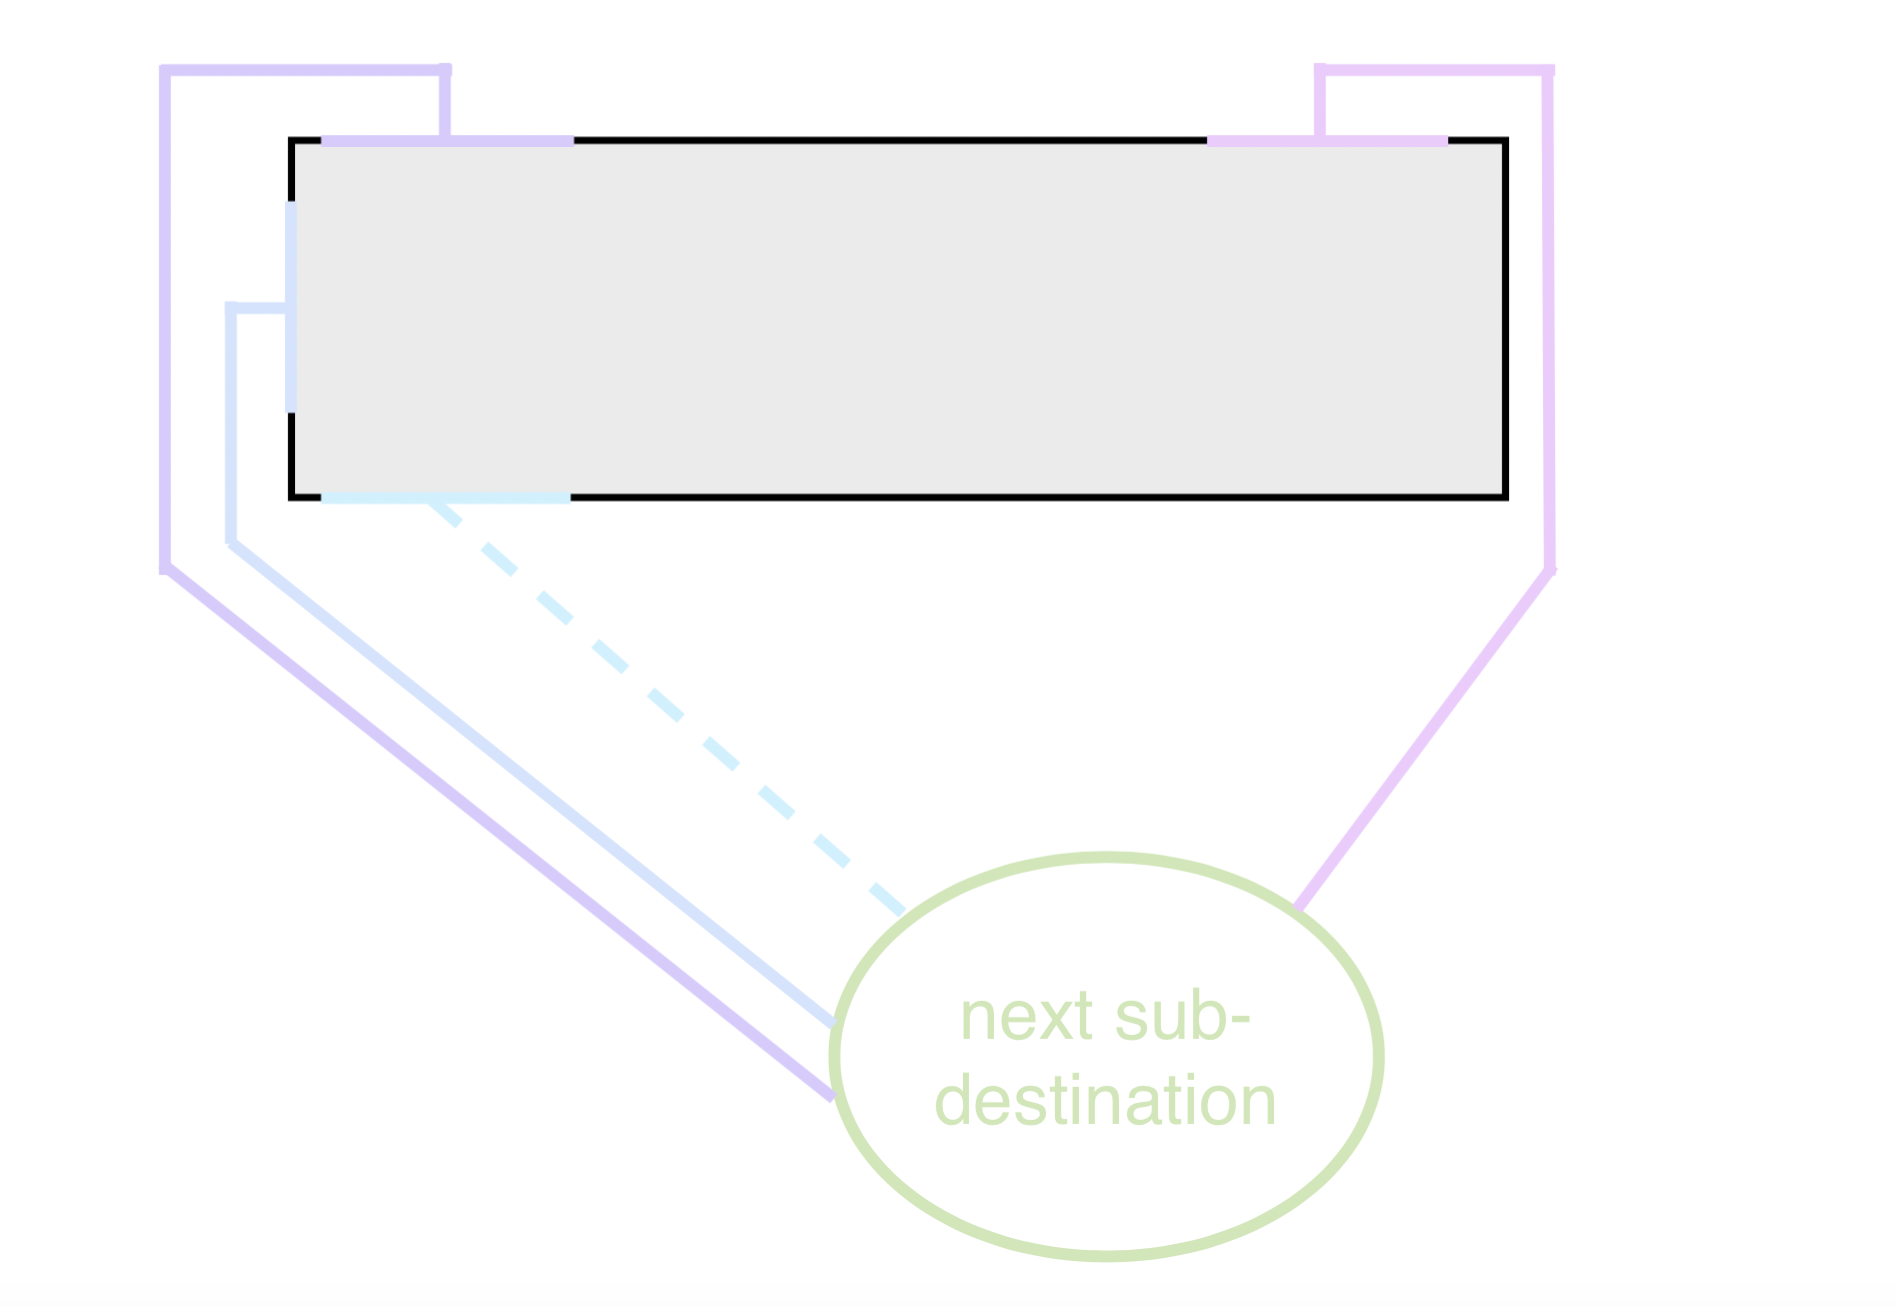
\includegraphics[width=0.8\linewidth]{figures/polygonal-chains-to-subdestination.png}
	\caption{Calcolo dei percorsi (rappresentati da linee spezzate, o \emph{polygonal chains}) congiungenti ogni varco di una walkable area con l’ellissi della prossima sotto-destinazione.}
	\label{fig:polygonal-chains-to-subdestination}
\end{figure}

\paragraph{Il sistema di pesi.} Ogni volta che un pedone entra in una nuova walkable area, gli archi incidenti su tale zona (ossia i passaggi tra questa e le zone adiacenti) vengono valutati sulla base delle informazioni spaziali disponibili. Il sistema di pesi, in letteratura \emph{weighting system} \cite{Andresen2018}, è usato per assegnare un peso ad ogni arco; quello con peso minimo sarà poi selezionato. Il calcolo del peso \(w\) di un arco \(e\) visibile viene effettuato come segue:
\begin{equation}\label{weighting-system}
w(e) = f_{volatile\ memory}\cdot f_{cognitive\ map}\cdot f_{final}
\end{equation}
dove \(f_{volatile\ memory}\) è il fattore che tiene conto della memoria volatile, calcolato come segue:
\begin{equation}
f_{volatile\ memory} = 2^{k}
\end{equation}
con \(k = 0,1,2,...\) che descrive quante volte la zona a cui l’arco conduce è stata visitata. Questo fattore è fondamentale quando la mappa cognitiva si rivela inutile in quanto favorisce l’esplorazione dell’ambiente. \(f_{cognitive\ map}\) è il fattore che tiene conto delle informazioni provenienti dalla mappa cognitiva, calcolato come segue:
\begin{equation}
f_{cognitive\ map} =
  \begin{cases}
    1 - 0.5^i     & \quad \text{if cognitive map is in use}\\
    1             & \quad \text{else}
  \end{cases}
\end{equation}
dove \(i = 1,2,3,...\) è il ranking assegnato all'arco che si sta valutando. Se la mappa cognitiva non è in uso perché non contiene informazioni utili, si avrà \(f_{cognitive\ map} = 1\) per ogni arco. Infine \(f_{final}\) è usato per tenere conto di eventuali uscite che vengono incontrate strada facendo, calcolato come segue: 
\begin{equation}
f_{final} =
  \begin{cases}
    \frac{1}{10}       & \quad \text{if edge leads to a final destination}\\
    1                  & \quad \text{else}
  \end{cases}
\end{equation}
Se l’arco che si sta valutando conduce a una zona che contiene una destinazione di interesse allora gli sarà assegnato \(f_{final} = 0.1\), altrimenti il peso assegnato è \(f_{final} = 1\). Si noti che questo richiedere di marcare alcune walkable areas dell'ambiente come finali, similmente a quanto già fatto per i landmark contenenti almeno una destinazione. Nel caso in cui venga incontrata un’uscita sconosciuta strada facendo, inoltre, l’eventuale percorso che si stava seguendo viene abbandonato. Le quantità costanti mostrate sono ricavate empiricamente in \cite{Andresen2018}. Quando più archi ottengono lo stesso peso e questo è il peso minimo, è necessario impiegare un qualche tipo di criterio per scegliere quale percorrere. In questi casi, viene scelto il varco più vicino alla posizione corrente del pedone, questo approccio è noto in letteratura come \emph{nearest door heuristic} \cite{Silvers2016, Andresen2016TheIO}. In futuro si potrebbero adottare strategie che meglio riproducono il comportamento umano, ad esempio è stato osservato che le persone tendono a muoversi sempre nello stesso verso a meno che la deviazione dalla direzione corrente fornisca una visibilità maggiore \cite{Peponis1990}.

\subsection{Ulteriori raffinamenti}
In questa sezione il sistema di pesi appena descritto viene raffinato ulteriormente, in modo da fornire ai pedoni simulati alcuni tratti ritenuti fondamentali. In particolare, vengono considerati due comportamenti:
\begin{itemize}
 \item \textbf{Evitare i vicoli ciechi}: In uno scenario di emergenza tipicamente i pedoni tendono ad evitare i vicoli ciechi per ovvie ragioni. Un semplice modo per indurre gli agenti simulati a fare lo stesso è aggiungere un fattore all'\cref{weighting-system} che aumenti il peso degli archi conducenti ad aree di questo tipo, ad esempio:
 
 \begin{equation}
 f_{impasse} =
  \begin{cases}
    10       & \quad \text{if pedestrian knows that the edge being}\\
             & \quad \text{weighted leads to an impasse}\\
    1        & \quad \text{else}
  \end{cases}
 \end{equation}
 Si noti che tale fattore è soggetto alla conoscenza del singolo: \(f_{impasse}\) assume valore massimo solo quando il pedone \emph{sa} che l'arco in esame conduce ad un vicolo cieco. In particolare, in questo caso viene fatto uso della memoria volatile: un arco conducente ad un'area senza uscite viene assegnato peso massimo solo dopo averne fatto esperienza, sarebbe infatti inaccurato impedire che pedoni con scarsa familiarità con l'ambiente incappino in zone di questo tipo. E' invece decisamente più realistico far sì che tali pedoni evitino di visitarle una seconda volta.
 \item \textbf{Evitare le congestioni}: La tendenza ad evitare aree congestionate è fondamentale in scenari d'emergenza, in quanto può influire significativamente su tempi e modi di evacuazione. In modo analogo a prima, si può aggiungere un fattore all'\cref{weighting-system} che aumenti il peso degli archi conducenti ad aree congestionate:
 \begin{equation}
 f_{congestion} = \frac{occupied\ area}{total\ area} + 1
 \end{equation}
 Il rapporto tra area occupata ed area totale della zona a cui l'arco in esame conduce corrisponde alla percentuale di occupazione di tale zona, o densità. Questo valore, originariamente appartenente all'intervallo \([0,1]\), viene mappato nell'intervallo \([1,2]\) in modo da evitare che in caso di densità nulla anche gli altri fattori vengano annullati.
 
 Si noti che la tecnica appena descritta non è che un'approssimazione del comportamento noto come \emph{congestion avoidance}. In una situazione di evacuazione reale, infatti, i pedoni coinvolti non solo tendono ad evitare aree  affollate, ma sono generalmente in grado di ricalcolare il proprio obbiettivo a fronte del movimento delle altre persone. Ad esempio, nel caso in cui il percorso verso l'uscita scelta risultasse troppo congestionato, un pedone reale potrebbe pensare di dirigersi verso un'uscita differente. In futuro, si potrebbe dotare i pedoni simulati di un tale comportamento.
\end{itemize}

In conclusione, il raffinamento dell'\cref{weighting-system} porta alla seguente formula:
\begin{equation}\label{weighting-system-refined}
w(e) = f_{volatile\ memory}\cdot f_{cognitive\ map}\cdot f_{final}\cdot f_{impasse}\cdot f_{congestion}
\end{equation}

\subsection{Automatizzare la generazione della mappa cognitiva}
\label{automatic-generation-cognitive-map}
Come già detto, l'obbiettivo di questa tesi è la realizzazione di pedoni con differenti gradi di conoscenza dell'ambiente circostante. E' stato spiegato che il livello di familiarità di un individuo con l'ambiente può essere variato aumentando o diminuendo il numero e la forma dei landmark presenti nella sua mappa cognitiva. In fase di scrittura di una simulazione, però, dover esplicitare la mappa cognitiva di ogni singolo individuo risulterebbe estremamente laborioso. Ciò che si vuole fare, invece, è permettere che tale struttura dati sia generata in modo automatico per ogni pedone, fornito il grafo dell'ambiente e il livello di familiarità dell'individuo. Di seguito viene presentato un semplice algoritmo per farlo, si procede come segue: viene scelta in modo casuale una percentuale di walkable areas pari al grado di familiarità del pedone, vengono scartate le zone la cui area risulta essere troppo piccola secondo una data soglia, in quanto difficilmente possono contenere un landmark. In ciascuna delle aree selezionate viene poi generata un'ellissi di dimensioni casuali ma completamente contenuta nella relativa zona. Per quanto riguarda le connessioni tra landmark, si produce un grafo in cui ogni ellissi è connessa ad ogni altra ellissi da essa raggiungibile, con un arco il cui peso è pari al numero di zone da attraversare per passare dall'una all'altra. Infine, viene generato un albero di copertura minimo di tale grafo; il significato di quest'ultima procedura è l'assunzione che i pedoni memorizzino la posizione di nuovi landmark rispetto a quella dei landmark già memorizzati più vicini, favorendo quindi relazioni spaziali tra landmark quanto più semplici possibili in termini di numero di aree da attraversare. Idealmente, più è alto tale numero più il percorso tra i due landmark è spezzato e, in un certo senso, complesso. Si noti che un albero di copertura per quanto minimo non necessariamente contiene un cammino minimo per ogni coppia di nodi del grafo, questo significa che un pedone con una familiarità totale con l'ambiente potrebbe non scegliere il percorso ottimo verso la sua destinazione. Questo può o meno essere ammissibile: da una parte è irrealistico pensare che una persona con conoscenza completa dell'ambiente non scelga il percorso migliore, dall'altra è pur vero che anche quando la nostra familiarità con un ambiente è alta tendiamo a percorrere le strade a cui siamo più avvezzi. In futuro, se si riterrà opportuno, si potrà modificare l'algoritmo in modo da generare un grafo contenente almeno un cammino minimo per ogni coppia di nodi.

\section{Progettazione}
In questa sezione i concetti introdotti finora vengono mappati nell'universo di Alchemist, ossia vengono rappresentati per mezzo delle entità che ne costituiscono il metamodello. Prima di entrare nel merito delle scelte progettuali fatte, però, è bene spiegare quanto già presente in Alchemist. Esistono tre tipi di pedone di crescente complessità creati partendo dal concetto di nodo:
\begin{itemize}
    \item \textbf{Pedone omogeneo}: un nodo con velocità di camminata e di corsa predefinite.
    \item \textbf{Pedone eterogeneo} un nodo con un sesso ed una età assegnati, dai quali sono determinate velocità, conformità alle regole ed attitudine ad aiutare.
    \item \textbf{Pedone cognitivo}: un pedone eterogeneo con delle emozioni, capace di influenzare e farsi influenzare dagli altri.
\end{itemize}
Esiste anche una varietà di azioni di steering create a partire dal concetto omonimo in Alchemist, e diverse reazioni che sfruttano e combinano queste azioni in modo differente. Per una più completa descrizione si veda il lavoro relativo\footnote{\url{https://amslaurea.unibo.it/19084/}}. 
\subsection{Grafo dell'ambiente e mappa cognitiva}
Grafo dell'ambiente e mappa cognitiva rivestono un ruolo principale nel processo di navigazione in quanto usati pervasivamente, entrambi sono rappresentabili come grafi i cui nodi possono essere riconducibili a figure convesse (poligoni in un caso, ellissi nell'altro), alcune delle quali necessitano di essere marcate come finali. Viste le somiglianze tra i due concetti, si è scelto di rappresentarli mediante una stessa interfaccia, si veda la \cref{fig:graph}.
\begin{figure}
	\centering
	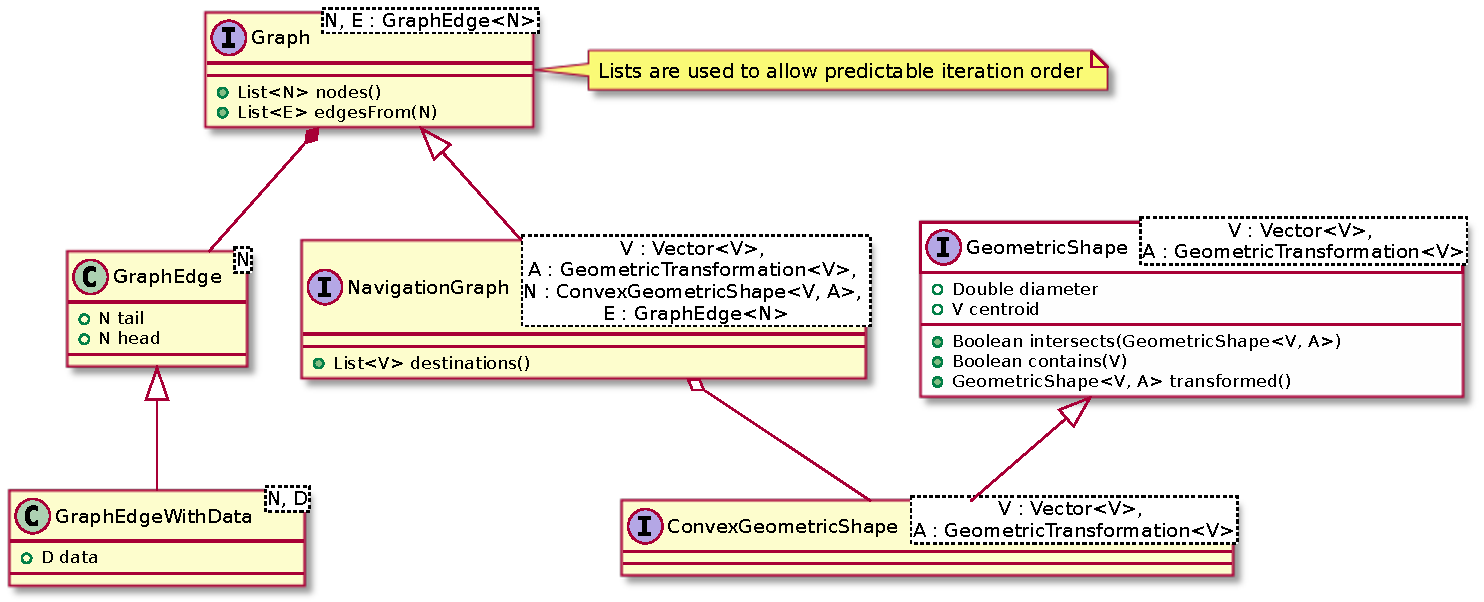
\includegraphics[width=\linewidth]{figures/graph.pdf}
	\caption{Diagramma delle classi UML che mostra la definizione del concetto di grafo di navigazione e la relativa gerarchia di interfacce. In giallo sono disegnati i componenti aggiunti, in bianco quelli già presenti.}
	\label{fig:graph}
\end{figure}
Un \texttt{NavigationGraph} altro non è che un grafo usato per scopi di navigazione, i cui nodi sono appunto figure convesse. In aggiunta, una tale struttura dati è in grado di memorizzare un insieme di destinazioni: le figure convesse contenenti queste destinazioni saranno marcate come finali. Questa scelta, rispetto alla semplice marcatura di alcune aree, permette ai pedoni di raggiungere l'esatta destinazione di interesse una volta avvistatala, ossia una volta entrati nella relativa area. Come si può vedere, nella definizione delle interfacce si è cercato di mantenere quanta più generalità possibile: l'interfaccia \texttt{Graph} modella un generico grafo diretto e dunque può essere riusata per altri scopi, si noti che mappa cognitiva e grafo dell'ambiente sono invece indiretti: un tale grafo può essere ottenuto semplicemente aggiungendo un arco nel verso opposto per ogni arco presente nella controparte diretta. Inoltre, l'interfaccia \texttt{NavigationGraph} non è vincolata ad un particolare spazio, dunque potrà essere riusata in simulazioni tridimensionali (o \emph{n-}dimensionali). Si sappia infatti che al momento Alchemist è dotato unicamente degli strumenti per simulazioni bidimensionali. Oltre a quanto mostrato, sono state aggiunte delle implementazioni assai triviali dei concetti di \texttt{Graph} e \texttt{NavigationGraph}, nonché altrettante classi \texttt{Builder} utilizzabili per ottenere tali oggetti secondo il paradigma definito dall'omonimo pattern\footnote{\url{https://en.wikipedia.org/wiki/Builder_pattern}}.

\subsection{Pedoni con capacità di orientamento}
Scopo di questa sezione è fornire ai pedoni descritti sopra la capacità di orientarsi. E' opportuno notare, però, che esiste una netta distinzione tra il concetto di pedone e il suo comportamento: il primo corriponde all'astrazione nella quale le informazioni spaziali come la mappa cognitiva sono contenute, il secondo consiste nell'elaborazione di tali informazioni ai fini dell'orientamento. Come già detto, in Alchemist i pedoni vengono definiti a partire dal concetto di nodo, mentre il loro comportamento corrisponde a una reazione. In questa sezione ci si concentrerà sulla nuova gerarchia di pedoni, mentre nella prossima si parlerà dei comportamenti associati. Fatta questa doverosa premessa, si può procedere alla progettazione: in \cref{fig:orienting-pedestrian-interfaces} viene mostrata la gerarchia di interfacce riguardanti il concetto di pedone, estesa con quanto descritto finora. Si è scelto di introdurre l'interfaccia \texttt{OrientingAgent}, in modo da non vincolare l'orientabilità ai pedoni umani. Come si può notare, inoltre, tale astrazione così come quelle da essa derivate non sono vincolate ad un particolare spazio, in modo da mantenere quanta più generalità possibile.
\begin{figure}
	\centering
	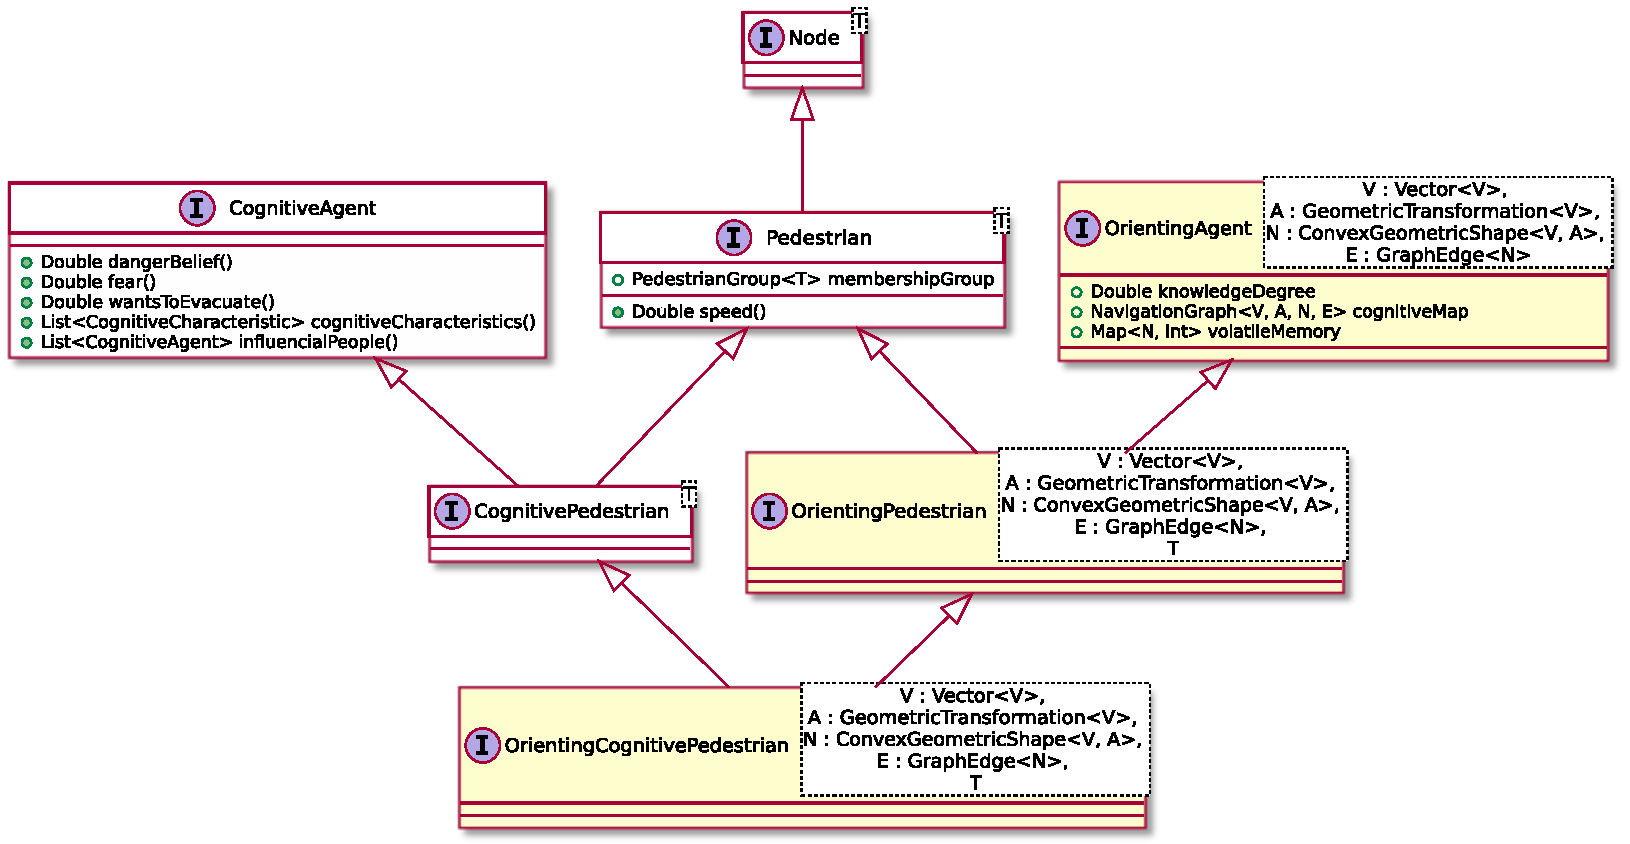
\includegraphics[width=\linewidth]{figures/orienting-pedestrian-interfaces.pdf}
	\caption{Diagramma delle classi UML che mostra la nuova gerarchia di interfacce relative al concetto di pedone. In giallo sono disegnati i componenti aggiunti, in bianco quelli già presenti.}
	\label{fig:orienting-pedestrian-interfaces}
\end{figure}
In \cref{fig:orienting-pedestrian-classes} viene mostrata la gerarchia di classi che realizzano tali interfacce, capostipite della gerarchia è la classe astratta \texttt{AbstractOrientingPedestrian}, che mantiene la massima generalità e contiene l'algoritmo descritto in \ref{automatic-generation-cognitive-map} per la generazione automatica della mappa cognitiva. Il solo compito lasciato alle sotto classi è la creazione dei landmark, via factory method\footnote{\url{https://it.wikipedia.org/wiki/Factory_method}}, in quanto dipendente dallo specifico spazio in cui il pedone si trova (ad esempio, in uno spazio tridimensionale è possibile che i landmark assumano la forma di ellissoidi anziché ellissi). La classe \texttt{OrientingPedestrian2D} definisce un pedone orientabile in un spazio euclideo bidimensionale ed implementa tale metodo; le sue sottoclassi realizzano delle versioni orientabili dei tipi di pedone già esistenti. A tal fine, \texttt{OrientingCognitivePedestrian2D} si compone dell'implementazione già presente di pedone cognitivo. Per evitare l'esplodere del numero di classi si è scelto di evitare la realizzazione di pedoni eterogenei orientabili, in quanto ottenibili dai pedoni cognitivi orientabili ignorandone la parte cognitiva. 
\begin{figure}
	\centering
	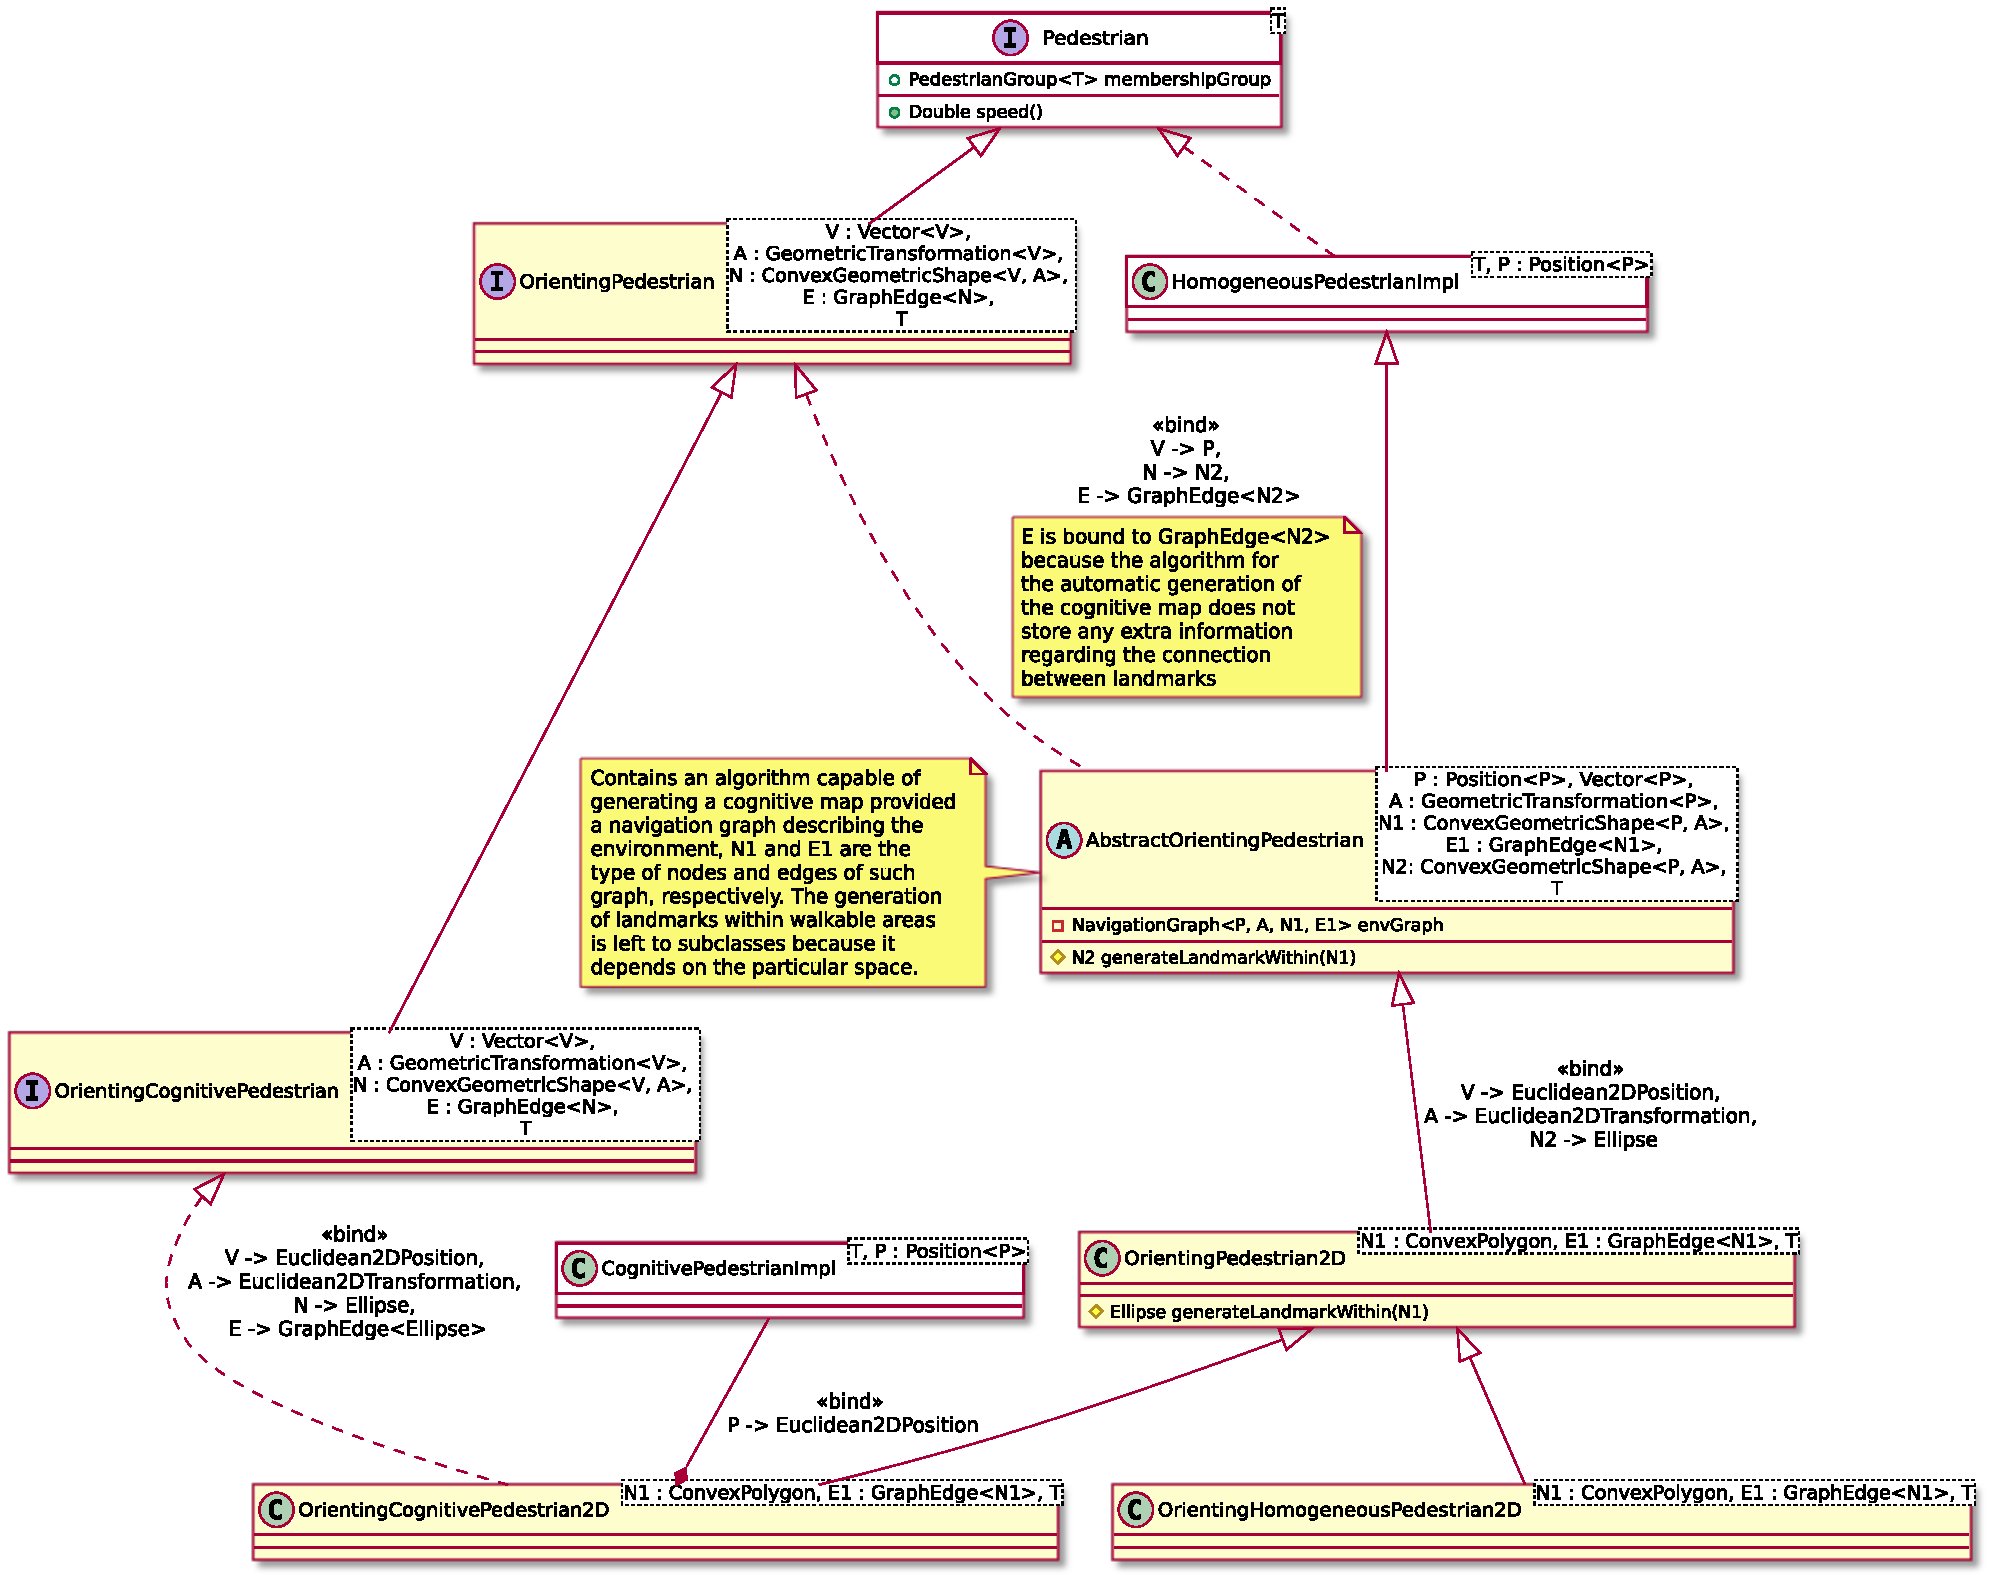
\includegraphics[width=\linewidth]{figures/orienting-pedestrian-classes.pdf}
	\caption{Diagramma delle classi UML che mostra la nuova gerarchia di classi relative al concetto di \texttt{OrientingPedestrian}. In giallo sono disegnati i componenti aggiunti, in bianco quelli già presenti.}
	\label{fig:orienting-pedestrian-classes}
\end{figure}

\subsection{Comportamento dei pedoni}
\label{design-orienting-behavior}
Scopo di questa sezione è definire una reazione capace di sfruttare le informazioni spaziali in possesso di un \texttt{OrientingPedestrian} ai fini della navigazione. 
\begin{figure}
	\centering
	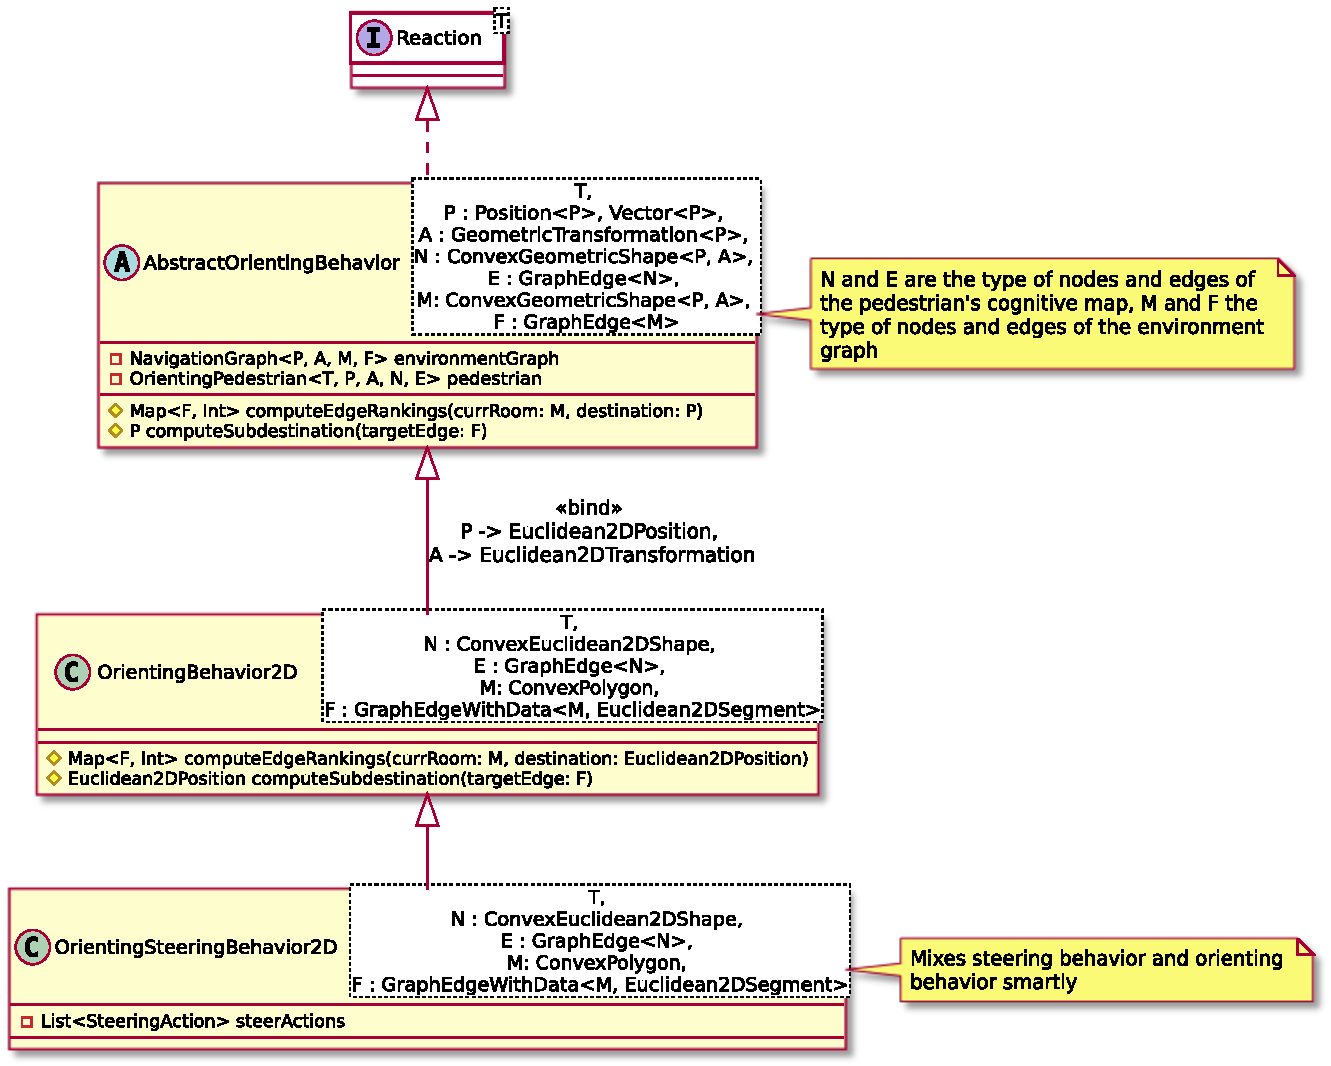
\includegraphics[width=0.8\linewidth]{figures/orienting-behavior.pdf}
	\caption{Diagramma delle classi UML che mostra la definizione delle reazioni costituenti il comportamento degli \texttt{OrientingPedestrian}. In giallo sono disegnati i componenti aggiunti, in bianco quelli già presenti.}
	\label{fig:orienting-behavior}
\end{figure}
In \cref{fig:orienting-behavior} è mostrata la gerarchia di classi relativa: ne è capostipite la classe astratta \texttt{AbstractOrientingBehavior}, che definisce il comportamento desiderato mantenendo la massima generalità e lasciando due compiti alle sotto classi, via template method\footnote{\url{https://en.wikipedia.org/wiki/Template_method_pattern}}, similmente a quanto già visto per \texttt{AbstractOrientingPedestrian}. In questo caso, ancor più che nel precedente, tale generalità viene al prezzo di una grande quantità di tipi parametrici, che però permettono di avere flessibilità massima. I compiti lasciati alle sotto classi sono i seguenti:
\begin{itemize}
    \item Classificazione dei varchi della zona corrente in base all'adeguatezza per il raggiungimento del prossimo landmark. Si tratta di quanto descritto in \ref{navigation-to-subdestination}: essendo una computazione fortemente geometrica, si è preferito lasciare l'onere dell'implementazione alla sotto classe \texttt{OrientingBehavior2D}. Questa assume uno spazio euclideo bidimensionale, e dunque ha la possibilità di usare varie funzioni di utilità che rendono il compito assai meno laborioso. In futuro, l'implementazione potrà essere spostata nella classe padre.
    \item Calcolo della posizione verso la quale muovere il pedone, dato il varco che si è scelto di attraversare. Questa procedura consiste nell'identificazione del punto appartenente al contorno della walkable area corrente, verso il quale il pedone deve dirigersi per spostarsi nella zona adiacente scelta. Per fare ciò naturalmente è necessario essere in possesso di maggiori informazioni riguardo la forma del varco scelto. Solitamente tali informazioni vengono memorizzate negli archi del grafo dell'ambiente, che rappresentano appunto i passaggi tra le varie walkable areas. Essendo che la classe astratta \texttt{AbstractOrientingBehavior} non fa assunzioni sul tipo di archi del grafo e la presenza di eventuali informazioni aggiuntive, tale compito è lasciato alle sotto classi. Come si può vedere, la classe derivata \texttt{OrientingBehavior2D} accetta invece un grafo dell'ambiente i cui archi contengono come informazione aggiuntiva un \texttt{Euclidean2DSegment}. Tale segmento, localizzato sul bordo di un poligono convesso, rappresenta proprio un passaggio tra questo e un poligono adiacente. Scelto un arco incidente sulla zona corrente, la procedura in esame otterrà il segmento associato a tale arco e identificherà il punto di questo che più è conveniente attraversare (può essere quello più vicino al pedone, o quello più vicino alla direzione del prossimo landmark da trovare).
\end{itemize}
Infine, è stata realizzata una reazione che combina azioni di steering e capacità di navigazione. L'implementazione di una classe \emph{ad hoc} si rende necessaria in quanto lasciare che le forze provenienti dai due comportamenti vengano combinate con una semplice somma può portare a situazioni assai poco realistiche. Si pensi al caso in cui più forze con verso opposto si annullano l'un l'altra: il pedone corre il rischio di rimanere immobile nonostante sottoposto a diversi stimoli. La classe \texttt{OrientingSteeringBehavior2D} si premura di combinare tali forze in modo da garantire che il pedone possa raggiungere la sua destinazione. Non si entra nel merito di come le forze vengono combinate in quanto i risultati ottenuti per quanto corretti sono ancora scarsi: i pedoni dotati di tale comportamento riescono si a raggiungere i propri obbiettivi, ma muovendosi in maniera poco realistica. In particolare, si verifica un fenomeno noto come \emph{shaking}, che causa movimenti a scatti. In futuro, si potranno adottare approcci più sofisticati e corretti alla combinazione delle forze rappresentati i diversi interessi di un individuo, in modo da rimuovere lo shaking.

\section{Implementazione}
\subsection{Metodologia di lavoro}
\subsubsection{Divisione in moduli}
Essendo Alchemist incentrato sulla modularità, si è seguito tale principio di divisione in moduli: le astrazioni relative ai pedoni orientabili sono state inserite nel modulo già esistente \texttt{alchemist-cognitive-agents}. La scelta è dovuta al fatto che i pedoni con capacità di navigazione cognitiva sono stati ritenuti a tutti gli effetti pedoni cognitivi. Le astrazioni relative al concetto di grafo e grafo di navigazione, invece, sono state inserite nel modulo \texttt{alchemist-implementationbase}, in quanto dotate di una certa generalità e riutilizzabili per diversi scopi.
\subsubsection{Divisione in package}
Tutte le astrazioni derivanti da entità del metamodello di Alchemist sono state organizzate in package seguendo la stessa struttura: è stata eseguita una netta divisione tra interfacce e implementazioni. In più, le implementazioni sono state divise in ulteriori package a seconda dell'entità del metamodello a cui fanno riferimento: nodo, azione o reazione. Per quanto riguarda le entità relative al concetto di grafo, sono state organizzate in un package omonimo, ed è stata seguita la medesima differenziazione tra interfacce ed implementazioni. Durante la scrittura di simulazioni in linguaggio YAML, tali accorgimenti permettono di specificare il tipo di un oggetto indicando esclusivamente il nome della classe, omettendo quindi l'intero package di appartenenza.
\subsection{Strumenti di sviluppo}
\subsubsection{Git} Git\footnote{\url{https://git-scm.com}} è un sistema di controllo di versione distribuito (DVCS) che permette di tenere traccia delle modifiche effettuate durante lo sviluppo di software. Tra le altre cose, git offre la possibilità di mantenere due versioni dello stesso progetto: una stabile e una in via di sviluppo; tale organizzazione risulta piuttosto flessibile per fronteggiare i problemi che solitamente si incontrano in fase di implementazione. Alchemist è sviluppato con la metodologia di lavoro nota come Gitflow\footnote{\url{https://nvie.com/posts/a-successful-git-branching-model/}}, che prevede che ogni componente del team di sviluppo abbia una propria copia del progetto principale: l'aggiunta di codice al repository centrale avviene per mezzo di \emph{pull requests}, con le quali un membro del team richiede che il suo codice sia aggiunto a tale repository.
\subsubsection{Gradle}
Gradle\footnote{\url{https://gradle.org}} è un sistema per l'automazione dello sviluppo software, la cui caratteristica principale è il supporto per sviluppi incrementali. In breve, esso è in grado di determinare quali porzioni del sistema software necessitano di essere ricostruite (fondamentalmente, quelle il cui codice è stato modificato), riducendo quindi significativamente il tempo di costruzione del progetto. Alchemist fa largo uso di tale strumento in quanto estremamente comodo soprattutto in progetti ad alto numero di dipendenze.
\subsubsection{Travis CI}
Travis CI\footnote{\url{https://travis-ci.org}} è un servizio di integrazione continua utilizzato per costruire e testare progetti software. Esso offre la possibilità di monitorare il comportamento del progetto su diversi sistemi operativi e con diverse configurazioni, permettendo quindi di tenere sotto controllo la retrocompatibilità ed il supporto multi-piattaforma di Alchemist, testandone il funzionamento con diverse versioni della JVM su tutti i principali sistemi operativi.
\subsubsection{Orchid}
Orchid\footnote{\url{https://orchid.run}} è uno strumento che permette la generazione automatica di pagine web statiche contenenti la documentazione relativa a classi e interfacce presenti in Alchemist (comunemente nota come API). Tale documentazione è estrapolata direttamente dal codice sorgente del progetto in maniera completamente automatica.
\subsubsection{Kotlin}
Kotlin\footnote{\url{https://kotlinlang.org}} è un linguaggio di programmazione general purpose, multi-paradigma (presenta sia caratteristiche tipiche della programmazione ad oggetti sia del paradigma funzionale), multi-piattaforma e open source; scelto per l'implementazione degli agenti orientabili in Alchemist. La sua caratteristica principale consiste nella completa interoperabilità con Java e con la Java Virtual Machine (JVM), che gli permette di sfruttare l'enorme quantità di librerie disponibili per quest'ultimo. Rispetto a Java, però, Kotlin risulta essere significativamente più conciso, cosa che ha permesso di accelerare notevolmente la fase di implementazione. Volendo citare concretamente uno dei vantaggi di Kotlin in tal senso, non si può non nominare le funzioni di estensione: come intuibile dal nome, queste permettono di estendere le funzionalità di particolari classi o interfacce senza intaccarne l'API. Durante lo sviluppo, è stato fatto largo uso di tale strumento per aggiungere al concetto di grafo un insieme di funzioni utili (come ad esempio un algoritmo per trovare un cammino minimo tra due nodi, e un altro per la generazione di un albero di copertura minimo), pur mantenendo un'interfaccia quanto più minimale possibile.
\subsection{Testing}
Ogni funzionalità non banale introdotta è stata corredata di un apposito insieme di test automatici, al fine di verificarne il corretto funzionamento e di impedire che modifiche future possano comprometterlo. Da una parte, per testare i componenti geometrici introdotti (quali ellissi e poligoni convessi) e gli algoritmi su grafo, è stato usato il framework JUnit\footnote{\url{https://junit.org}}. Per i test sui pedoni orientabili, invece, è stata usata la libreria Kotest (o KotlinTest)\footnote{\url{https://github.com/kotest/kotest}}. In particolare, per testare in modo automatico la correttezza del comportamento dei pedoni orientabili, sono state create simulazioni \emph{ad hoc} che durante i test vengono caricate ed eseguite. La situazione finale di ogni simulazione viene confrontata con la situazione prevista per determinare la correttezza o meno del comportamento dei pedoni.

%----------------------------------------------------------------------------------------
\chapter{Risultati ottenuti}
\label{chap:results}
Di seguito vengono presentati quattro casi di studio con l'obbiettivo di evidenziare le potenzialità dei pedoni dotati di capacità di navigazione cognitiva. I primi tre coinvolgono un singolo pedone alle prese con uno stesso ambiente, ma con un livello di familiarità via via decrescente. L'ultimo caso mostra la tendenza dei pedoni orientabili ad evitare aree congestionate.
%----------------------------------------------------------------------------------------
\section{Conoscenza completa dell'ambiente}
\label{complete-knowledge-case-study}
Un singolo pedone dotato di conoscenza completa dell'ambiente è inserito all'interno di un edificio dalla planimetria non banale. Inoltre, una destinazione di interesse è collocata diverse stanze oltre la posizione iniziale del pedone, in modo che raggiungerla con un percorso diretto sia impossibile. Si noti che un qualsiasi pedone non orientabile proverebbe a raggiungerla proprio percorrendo la direzione che lo collega in linea d'aria a tale destinazione. Si noti anche che in quanto la conoscenza del pedone simulato è completa, questo sicuramente è a conoscenza della posizione della destinazione (o meglio, la sua mappa cognitiva conterrà senz'altro un landmark speciale che racchiude tale destinazione). Ciò che ci aspetta da un individuo del genere è che intraprenda il percorso più corto possibile verso l'obbiettivo, senza incappare in vicoli ciechi o rimanere bloccato in alcun modo. In \cref{fig:complete-knowledge} si può osservare che il pedone compie proprio un percorso del genere.
\begin{figure}
	\centering
	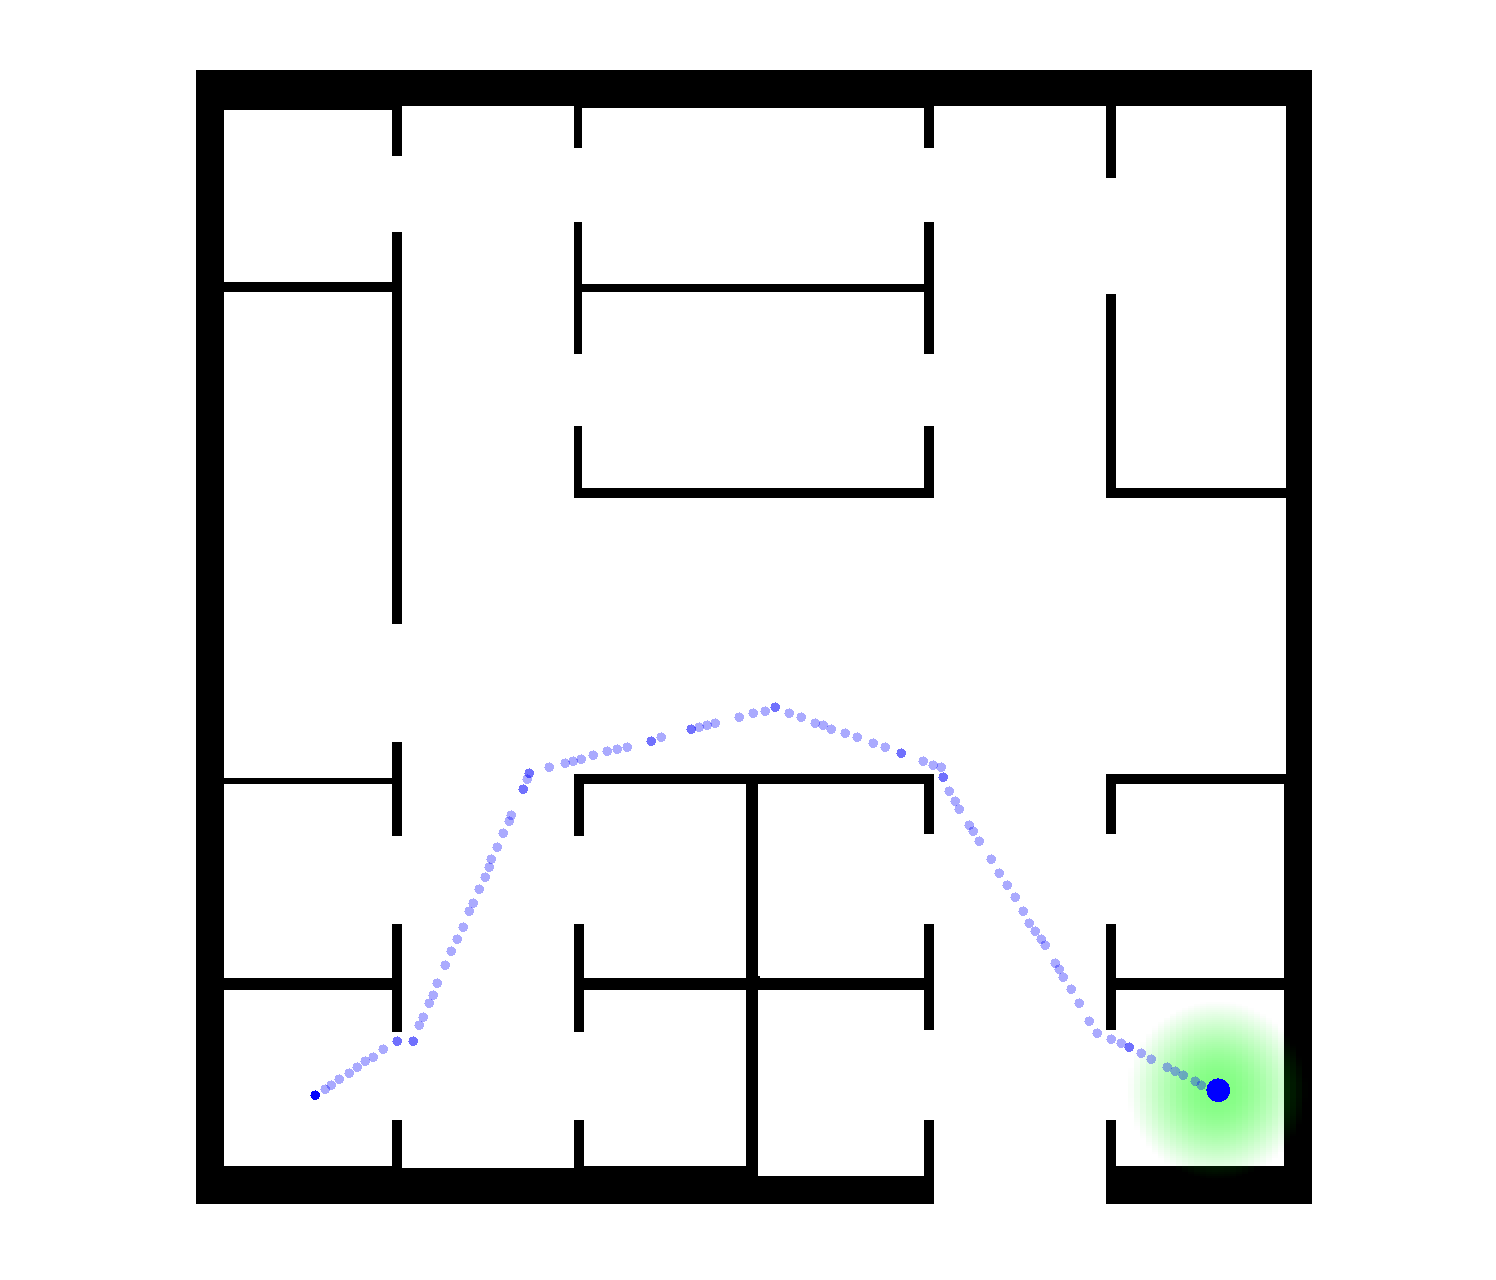
\includegraphics[width=0.7\linewidth]{figures/complete-knowledge.png}
	\caption{In blu è disegnato il percorso intrapreso da un pedone orientabile con conoscenza completa dell'ambiente verso la destinazione marcata di verde.}
	\label{fig:complete-knowledge}
\end{figure}
\section{Conoscenza parziale dell'ambiente}
\label{partial-knowledge-case-study}
Un singolo pedone dotato di conoscenza parziale dell'ambiente (30\%) è inserito nel medesimo edificio della simulazione precedente. Allo stesso modo, una destinazione di interesse è collocata diverse stanze oltre la posizione iniziale del pedone. Questa volta il comportamento dell'individuo simulato è fortemente dipendente dalle informazioni presenti nella sua mappa cognitiva: non necessariamente, infatti, questa conterrà la posizione della destinazione di interesse. In più, i suoi movimenti saranno tanto più sicuri (o tanto migliori) quanta è maggiore la sua familiarità con la porzione di ambiente che sta attraversando. In \cref{fig:partial-knowledge-cognitive-map} si può osservare la mappa cognitiva del pedone simulato: questa contiene un landmark che racchiude la posizione della destinazione di interesse (collocata come nella simulazione precedente nella stanza in basso a destra), e generalmente è ricca di informazioni riguardanti la porzione di edificio ad est. E' però sprovvista di qualsivoglia informazione riguardo la porzione di edificio in cui il pedone si trova inizialmente.
\begin{figure}
	\centering
	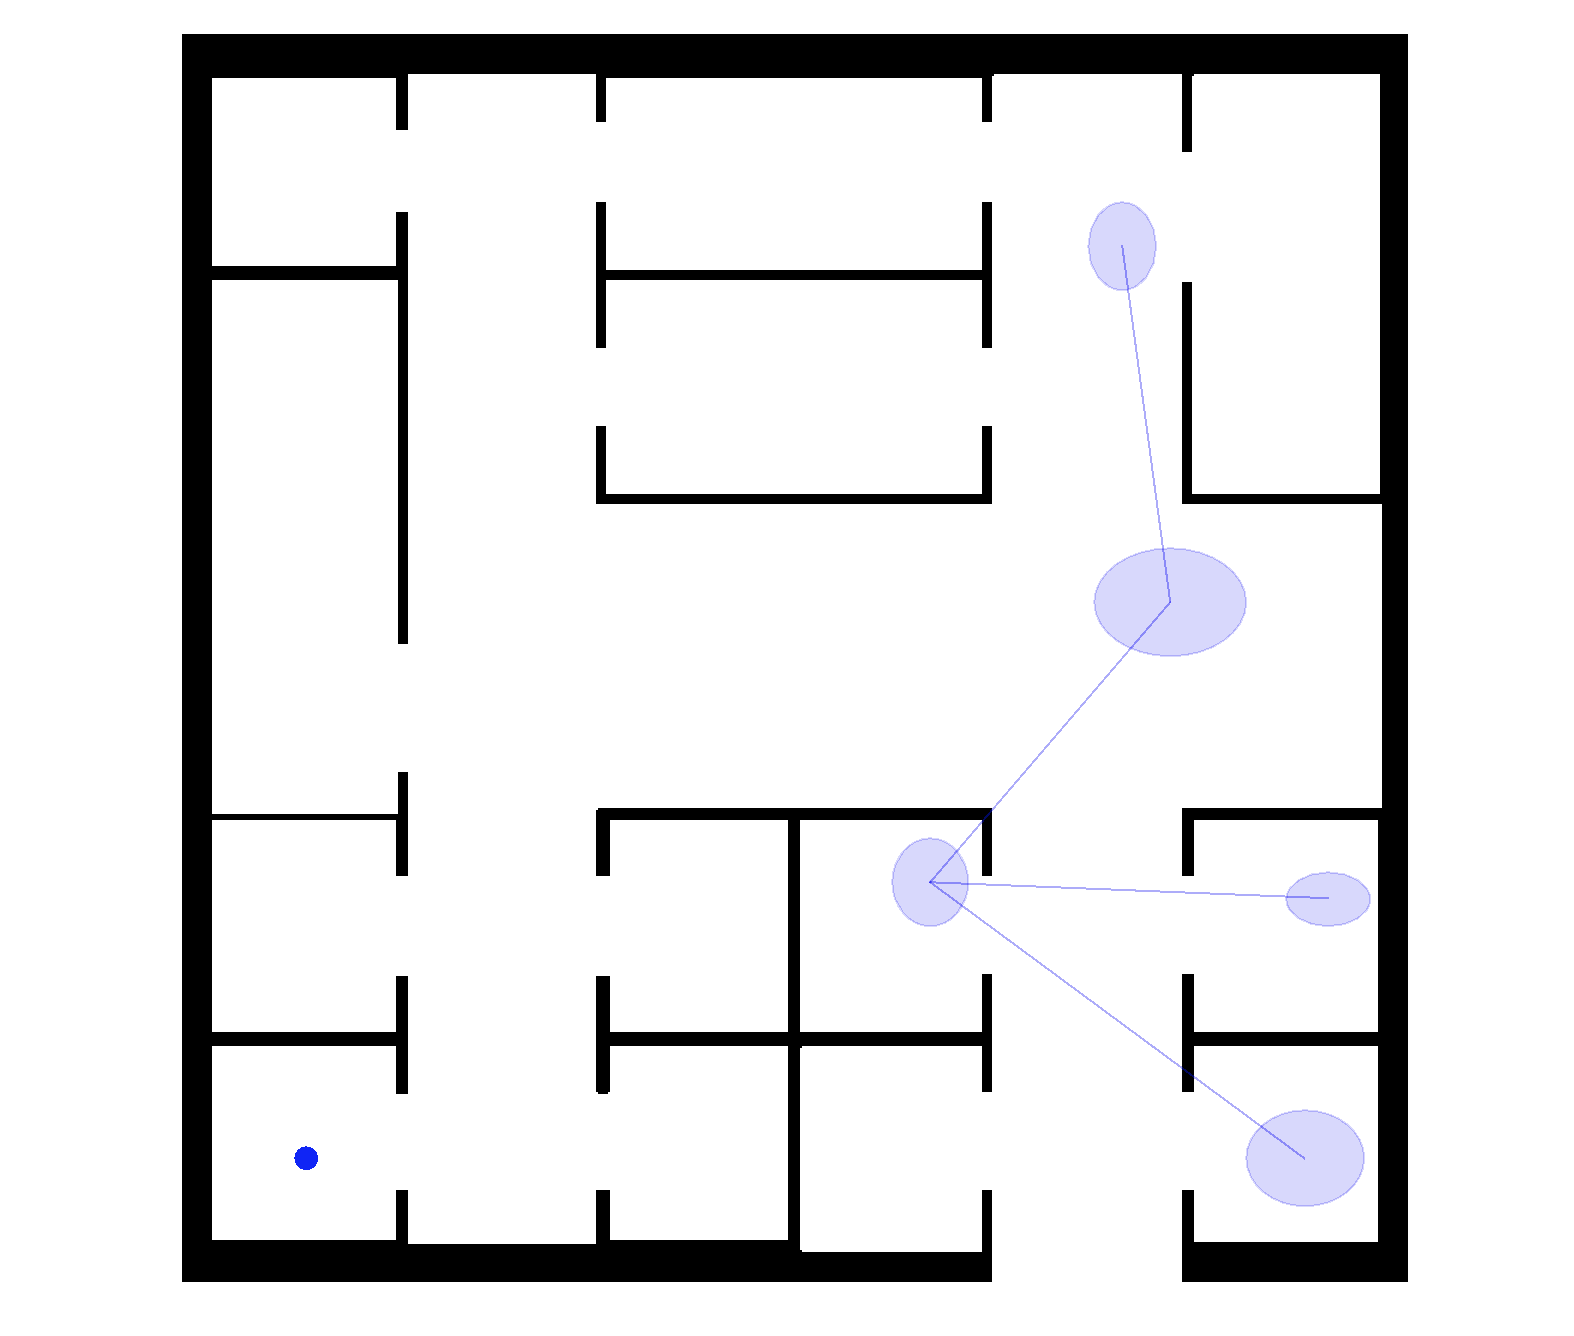
\includegraphics[width=0.7\linewidth]{figures/partial-knowledge-cognitive-map.png}
	\caption{In blu è disegnata la mappa cognitiva del pedone orientabile con conoscenza parziale simulato nel caso di studio corrispondente. Si può osservare sia la forma ellittica dei landmark, sia le connessioni tra questi. Si ricorda che la mappa cognitiva in questione memorizza unicamente un'informazione booleana riguardo la connessione tra due landmark, tale dato in figura è mostrato disegnando un segmento tra i baricentri dei landmark connessi.}
	\label{fig:partial-knowledge-cognitive-map}
\end{figure}
In \cref{fig:partial-knowledge} si può osservare il percorso compiuto dall'individuo simulato: come preventivato, questo incappa in diversi vicoli ciechi all'inizio della simulazione, a causa della scarsa familiarità con la porzione d'ambiente corrispondente. Si noti inoltre che tali stanze senza uscite vengono visitate dal pedone un'unica volta: non appena questo entra in una zona del genere (e dunque percepisce l'assenza di altre uscite), questa viene abbandonata e non verrà più visitata. Infine, una volta che il pedone riesce ad arrivare nella porzione di edificio più familiare, trova immediatamente un buon percorso verso la destinazione di interesse.  
\begin{figure}
	\centering
	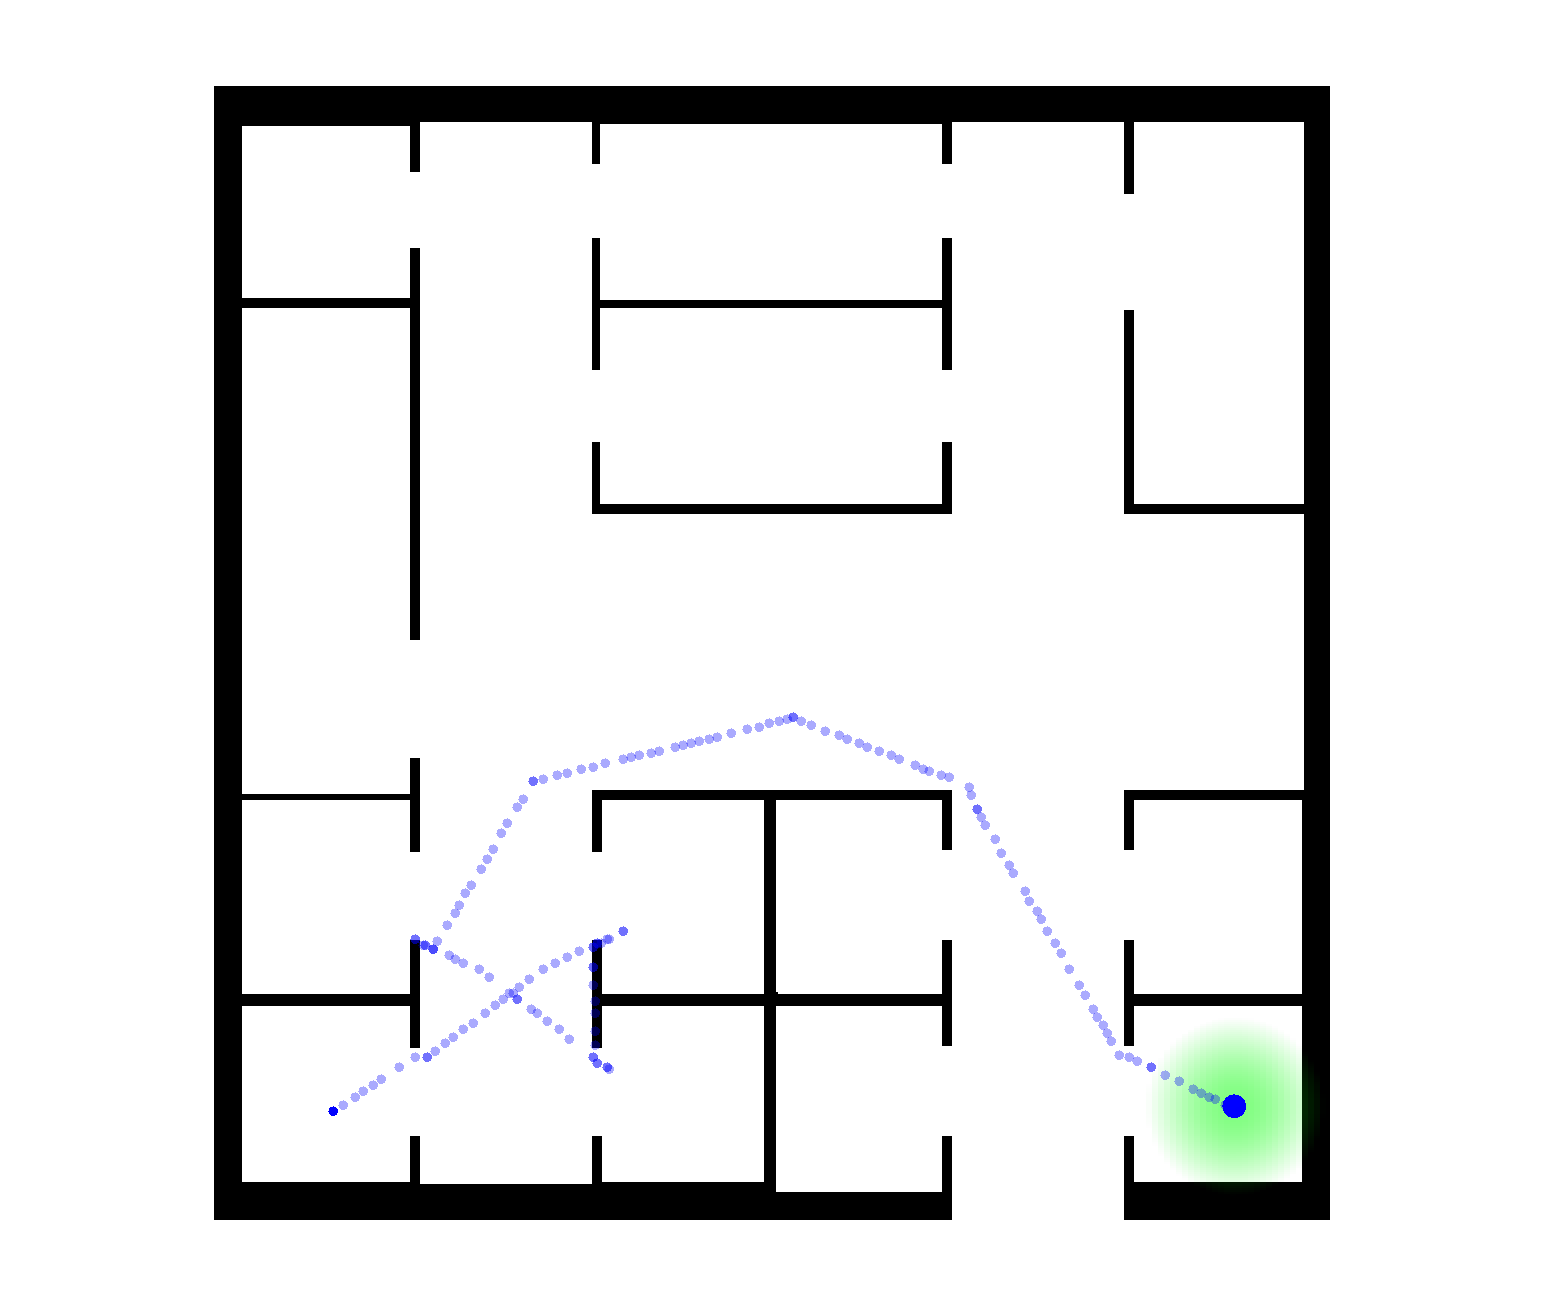
\includegraphics[width=0.7\linewidth]{figures/partial-knowledge.png}
	\caption{In blu è disegnato il percorso intrapreso da un pedone orientabile con conoscenza parziale dell'ambiente (30\%) verso la destinazione marcata di verde.}
	\label{fig:partial-knowledge}
\end{figure}
\section{Nessuna conoscenza dell'ambiente}
\label{no-knowledge-case-study}
Un pedone con familiarità dell'ambiente pari a zero è inserito nel medesimo edificio delle due simulazioni precedenti. Similmente a prima, una destinazione di interesse è collocata diverse stanze oltre la posizione iniziale del pedone. Essendo l'individuo simulato sprovvisto di alcun tipo di conoscenza pregressa riguardo l'edificio, sicuramente non sarà a conoscenza della posizione della destinazione di interesse (in particolare, la sua mappa cognitiva sarà del tutto vuota). Nonostante questo, essendo dotato di capacità di orientamento, ci si aspetta che prima o poi il pedone riesca a trovare tale destinazione, specie in virtù del comportamento di esplorazione di cui si è parlato in \ref{weighting-system}. In \cref{fig:no-knowledge} si può osservare il percorso compiuto dall'individuo simulato: come preventivato, questo deve esplorare numerose stanze e incappare in diversi vicoli ciechi prima di trovare la destinazione ed arrestarsi.
\begin{figure}
	\centering
	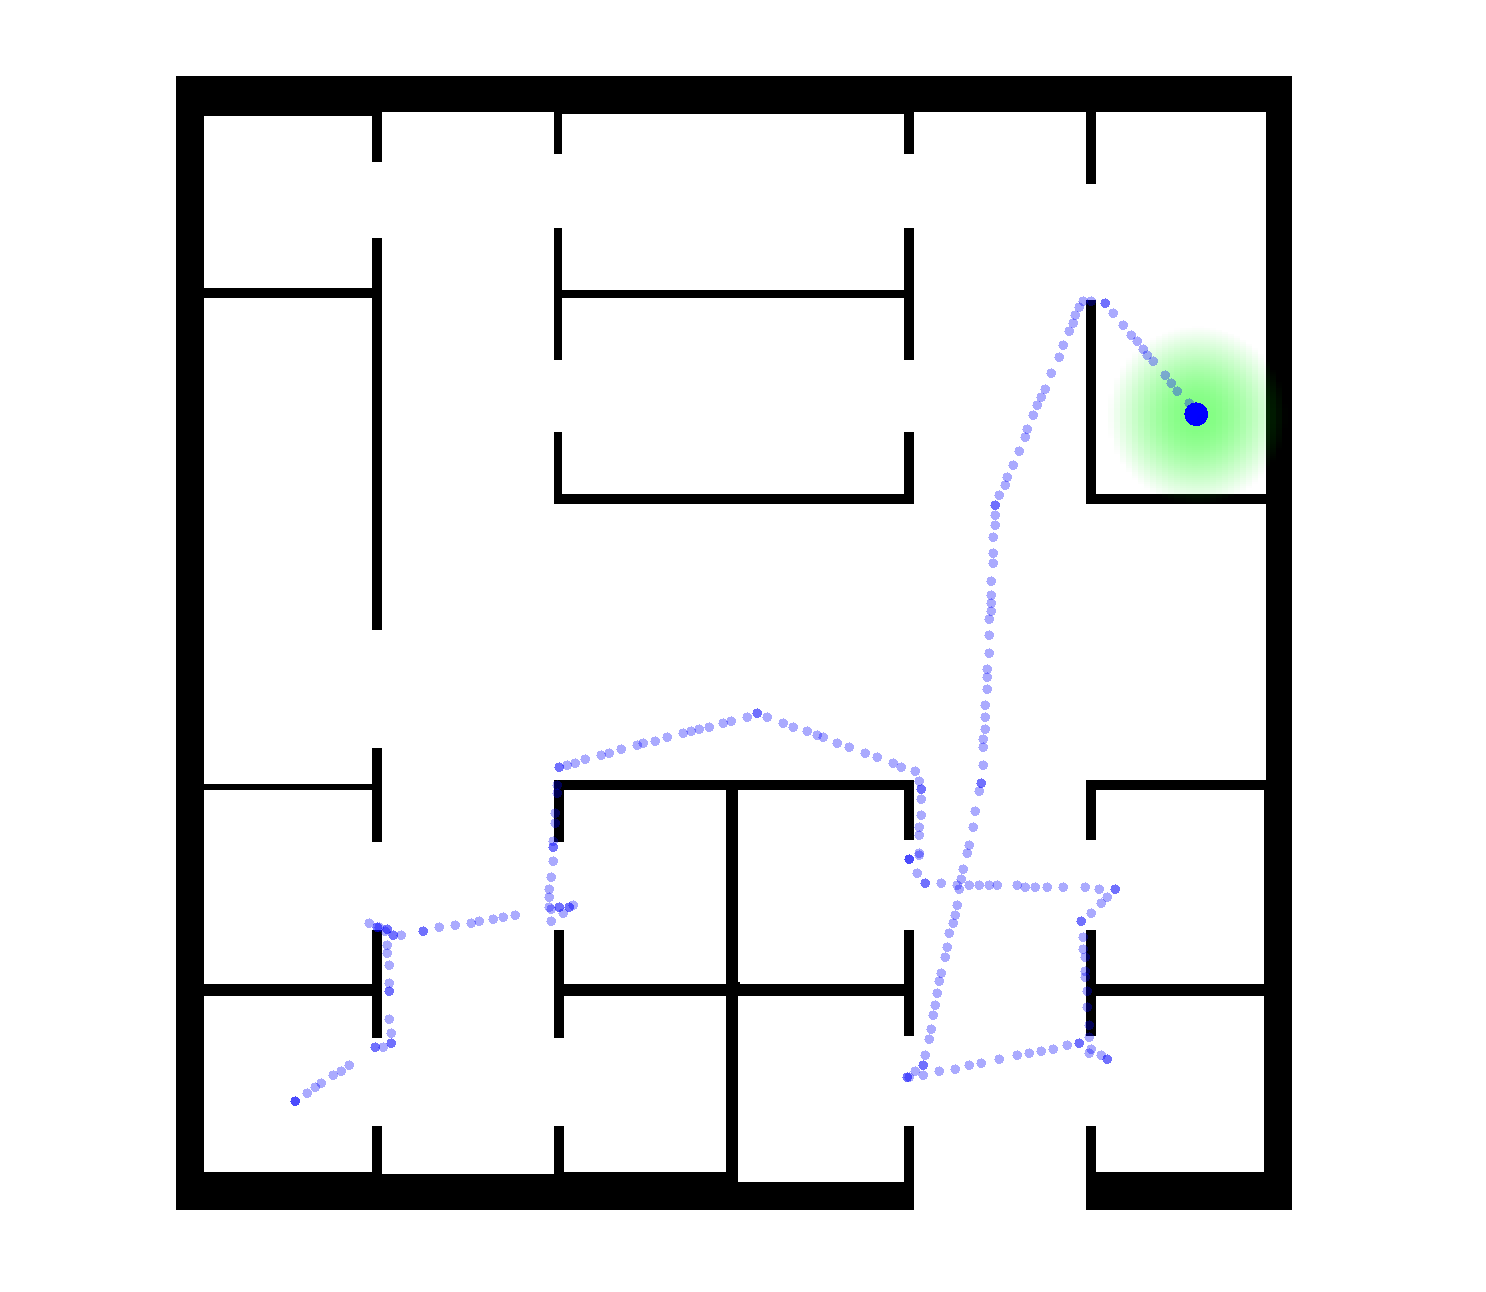
\includegraphics[width=0.7\linewidth]{figures/no-knowledge.png}
	\caption{In blu è disegnato il percorso intrapreso da un pedone orientabile sprovvisto di alcun tipo di conoscenza pregressa dell'ambiente verso la destinazione marcata di verde. In particolare, è apprezzabile la tendenza ad esplorare l'ambiente al fine di trovare la destinazione di interesse.}
	\label{fig:no-knowledge}
\end{figure}
\section{Evitare le congestioni}
\label{congestion-avoidance-case-study}
Per questo caso di studio cento trenta pedoni orientabili dotati di conoscenza completa dell'ambiente sono collocati in un edificio dalla planimetria assai più semplice della precedente, ma che comunque permette di intraprendere diverse strade verso la destinazione di interesse; la si può vedere in \cref{fig:congestion-avoidance-1}. In prima istanza, viene effettuata una simulazione con lo scopo osservare le scelte dei pedoni orientabili in assenza di congestioni (se non quelle formate da loro stessi). Ciò che ci si aspetta è che tutti o quasi gli individui simulati compiano il percorso più breve possibile verso la destinazione di interesse, ossia quello che passa per il corridoio più a nord. In \cref{fig:congestion-avoidance-1} si può vedere come la quasi totalità dei pedoni si attiene a questa scelta. I pochi che optano per strade diverse lo fanno o per evitare la congestione formatasi nel primo corridoio, o per via di quanto detto in \cref{automatic-generation-cognitive-map}. 
\begin{figure}
	\centering
	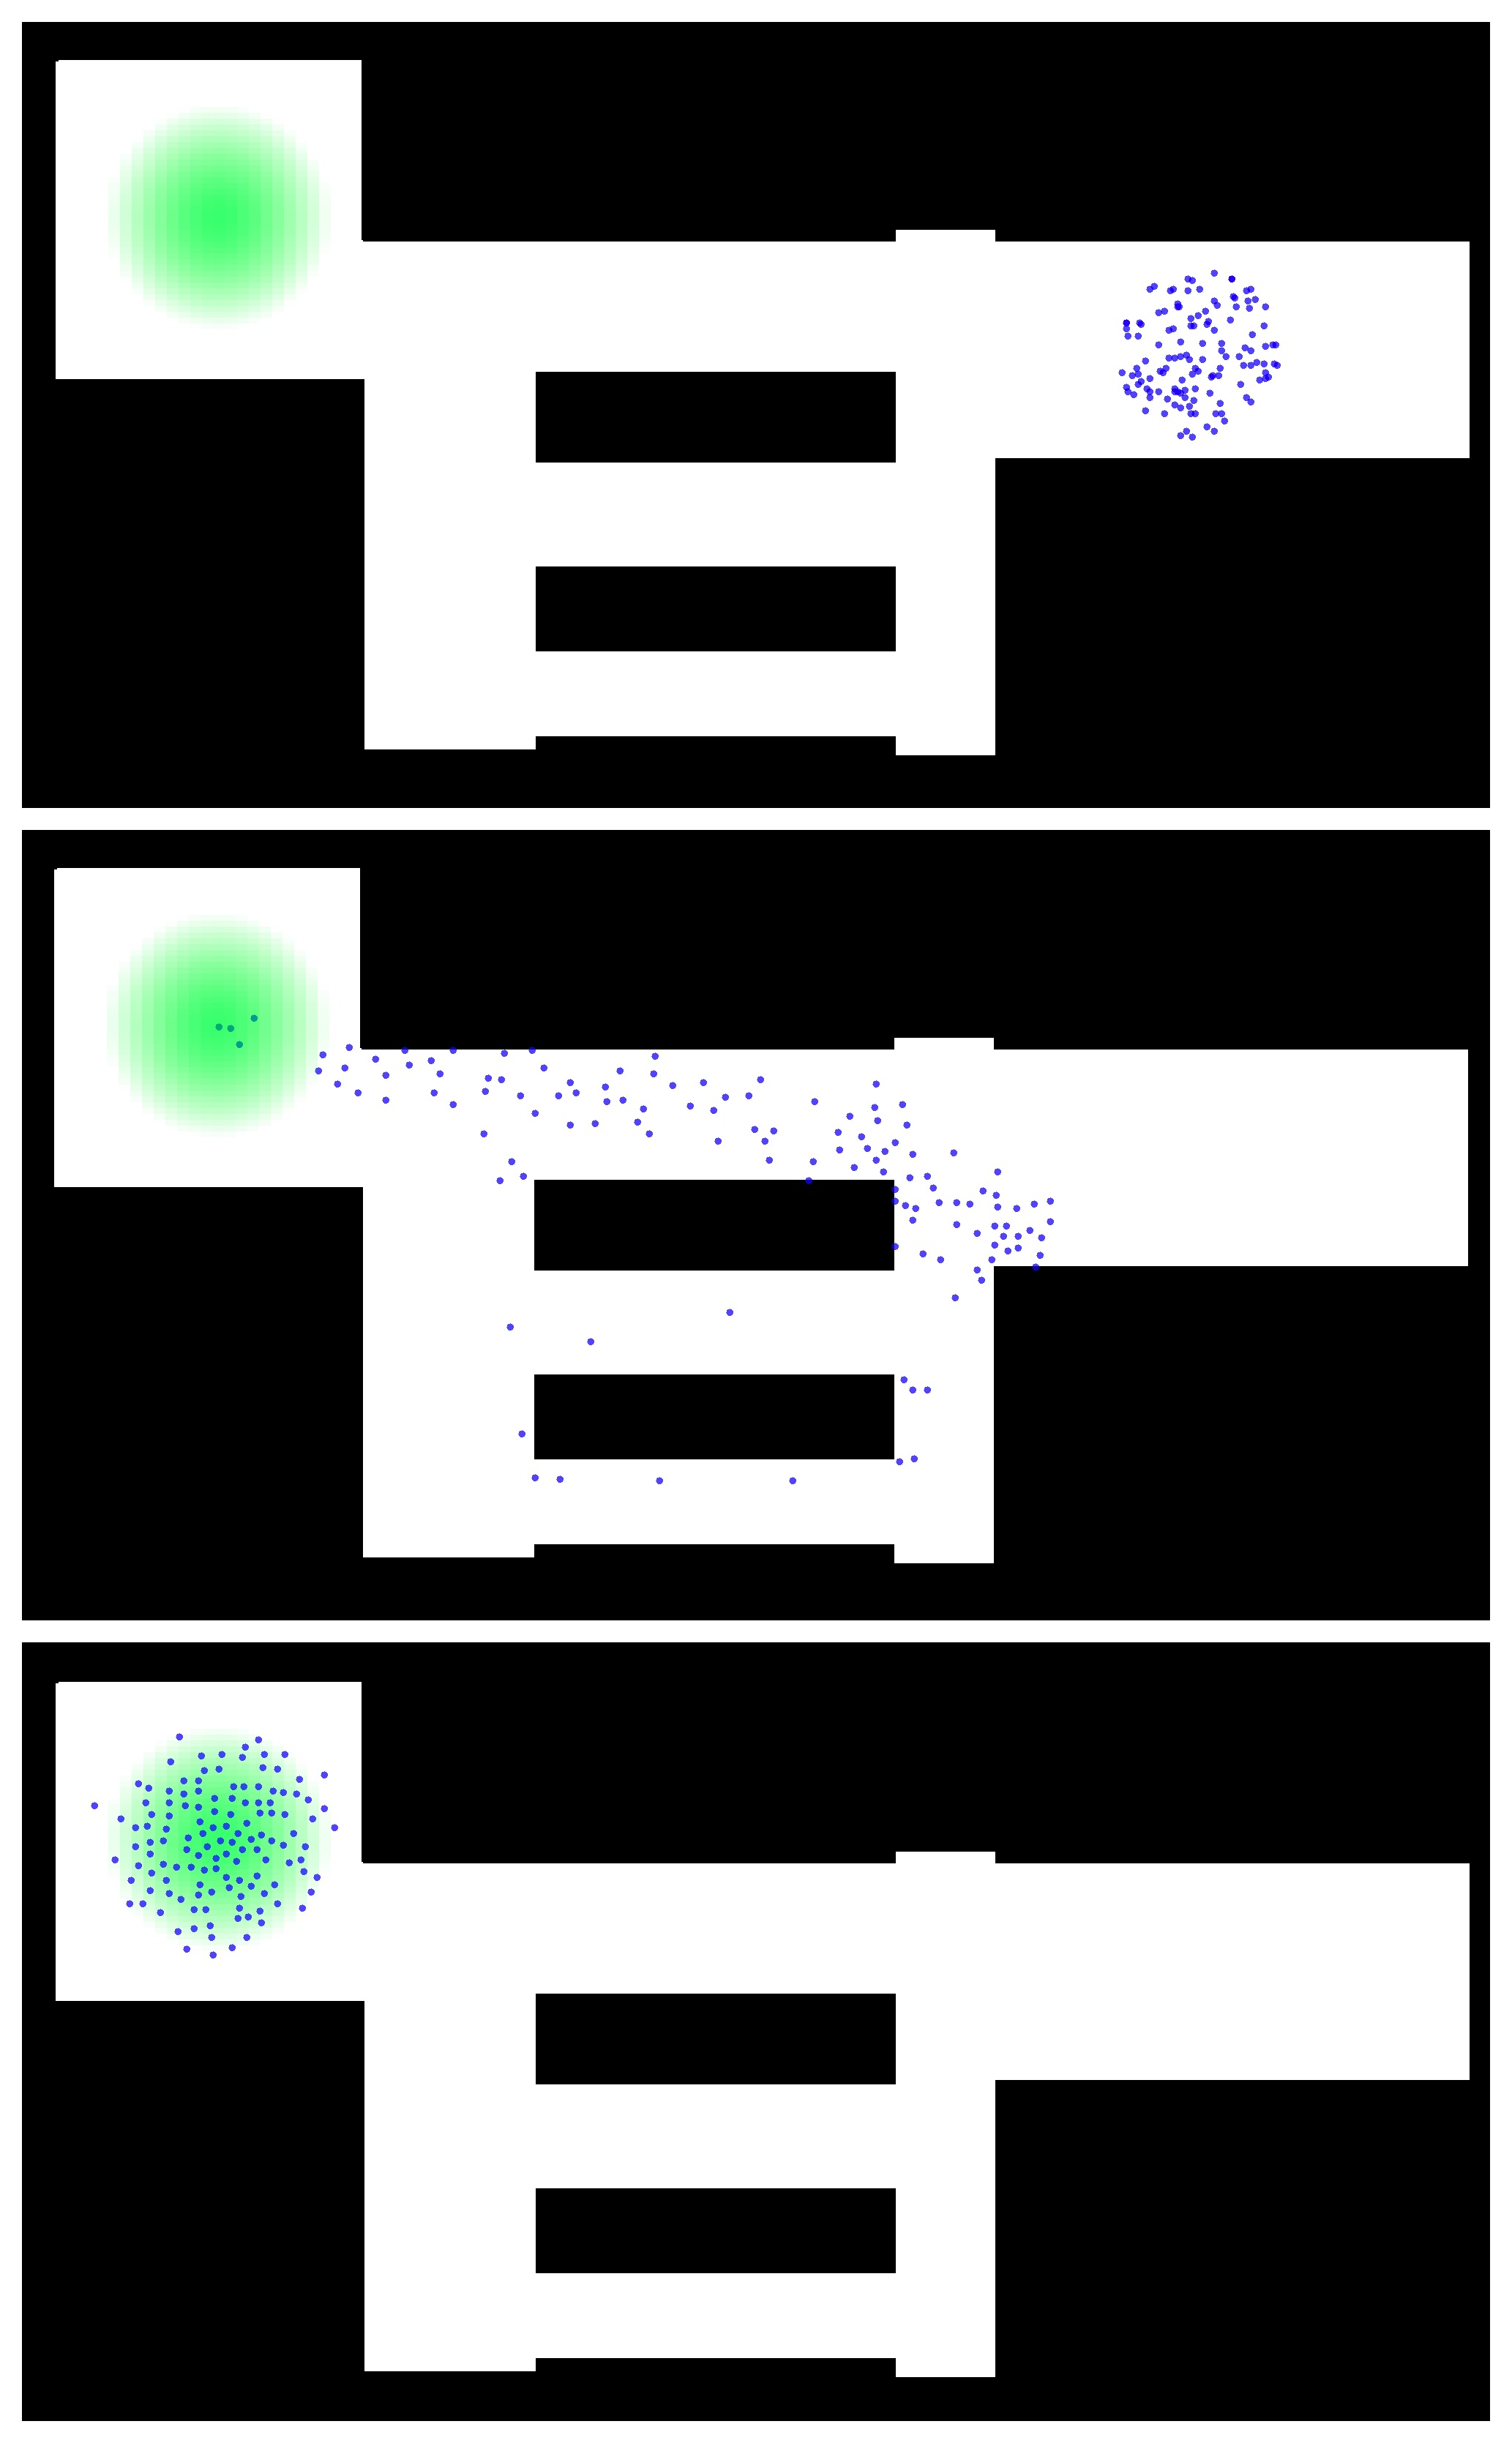
\includegraphics[width=0.5\linewidth]{figures/congestion-avoidance-1.png}
	\caption{Istantanee della situazione a inizio, metà e fine della prima simulazione di \emph{congestion avoidance}. In blu sono disegnati i pedoni orientabili coinvolti, in verde la destinazione di interesse.}
	\label{fig:congestion-avoidance-1}
\end{figure}
Fatto ciò, la simulazione viene ripetuta con una variazione: una gran quantità di pedoni senza capacità di locomozione viene collocata nei due corridoi più a nord, in modo da causare un ingente congestione nei due percorsi più brevi. Ciò che ci aspetta, è che i pedoni orientabili scelgano il percorso meno congestionato verso la destinazione. In \cref{fig:congestion-avoidance-2} si può osservare che la totalità degli individui dotati di capacità di navigazione cognitiva compie proprio tale percorso.
\begin{figure}
	\centering
	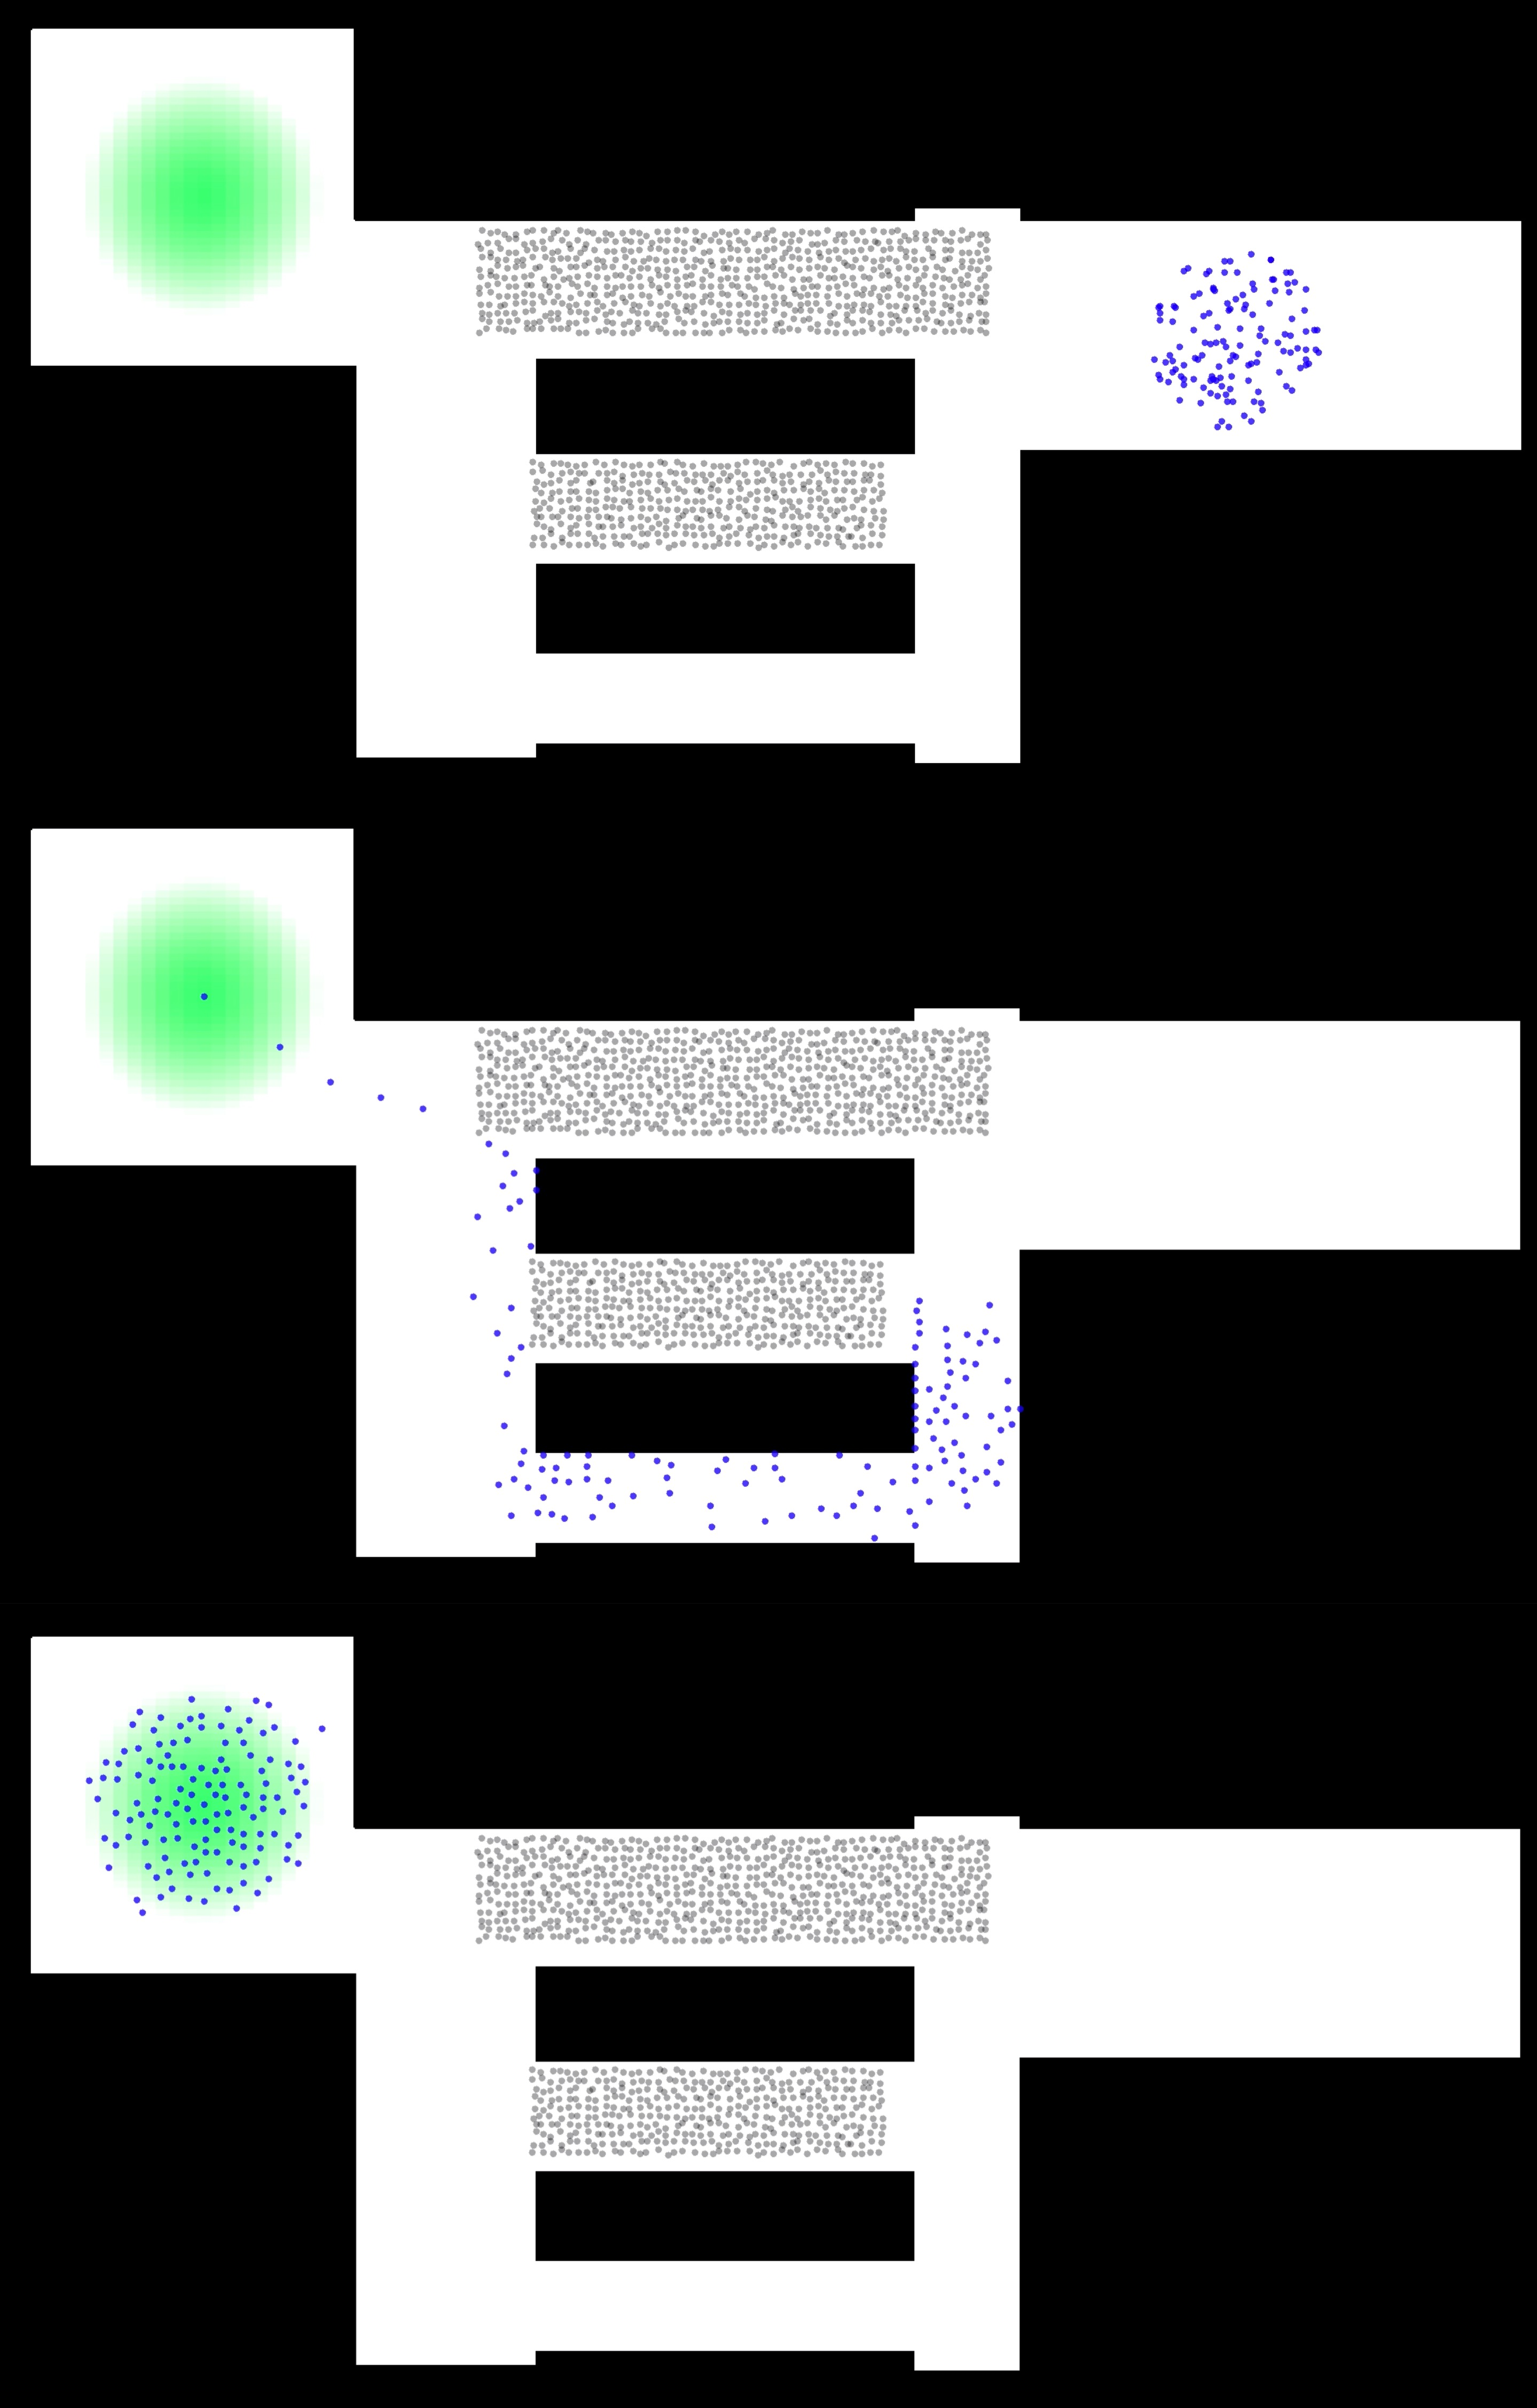
\includegraphics[width=0.5\linewidth]{figures/congestion-avoidance-2.png}
	\caption{Istantanee della situazione a inizio, metà e fine della seconda simulazione di \emph{congestion avoidance}. In blu sono disegnati i pedoni orientabili coinvolti, in grigio i pedoni sprovvisti di capacità locomotorie, in verde è marcata la destinazione di interesse.}
	\label{fig:congestion-avoidance-2}
\end{figure}

%----------------------------------------------------------------------------------------
\chapter{Conclusioni e sviluppi futuri}
\label{chap:conclusions}
%----------------------------------------------------------------------------------------
I pedoni realizzati presentano il comportamento desiderato e sono sufficientemente semplici (in termini di complessità computazionale) da essere utilizzati in simulazioni ad alto numero di agenti. Detto ciò, ad ora presentano due principali svantaggi: il primo consiste nella mancanza di una tecnica affidabile e realistica per la combinazione di comportamenti di steering e navigazione cognitiva, come menzionato in \ref{design-orienting-behavior}. Finché Alchemist non sarà dotato di una tale tecnica, difficilmente si potrà dotare i pedoni simulati di entrambi gli aspetti (o meglio, lo si potrà fare ma ottenendo movimenti poco realistici, come già detto). Il secondo svantaggio sta nel fatto che il modello scelto è fortemente dipendente dalla divisione dell'ambiente in poligoni convessi; in particolare, una divisione realistica è indispensabile per osservare un comportamento tale. Questo è dovuto perlopiù alle abilità percettive dei pedoni realizzati: essi sono in grado di percepire tutta e sola la walkable area in cui si trovano, ne percepiscono cioè la forma e i passaggi alle aree adiacenti (in realtà, sono in grado anche di valutare la congestione aldilà di un varco, ma questo è ritenuto del tutto accettabile). Si pensi dunque al caso in cui i poligoni generati siano eccessivamente grandi o oltremodo piccoli: i pedoni simulati avrebbero abilità percettive del tutto fuori luogo, e tali sarebbero i loro movimenti. Si veda la figura \cref{fig:envgraphs}, essa mostra due grafi di navigazione: uno generato in maniera semi automatica (dunque con l'aiuto dell'uomo), l'altro generato in maniera completamente automatica. Si può facilmente notare che i poligoni del secondo grafo sono notevolmente più frammentari e in generale offrono una descrizione dell'ambiente ritenuta peggiore. Si pensi infatti di voler simulare il movimento di pedoni orientabili attraverso le aree di cui si compone tale grafo: è facile immaginare che il comportamento risultante sarebbe poco realistico.
\begin{figure}
	\centering
	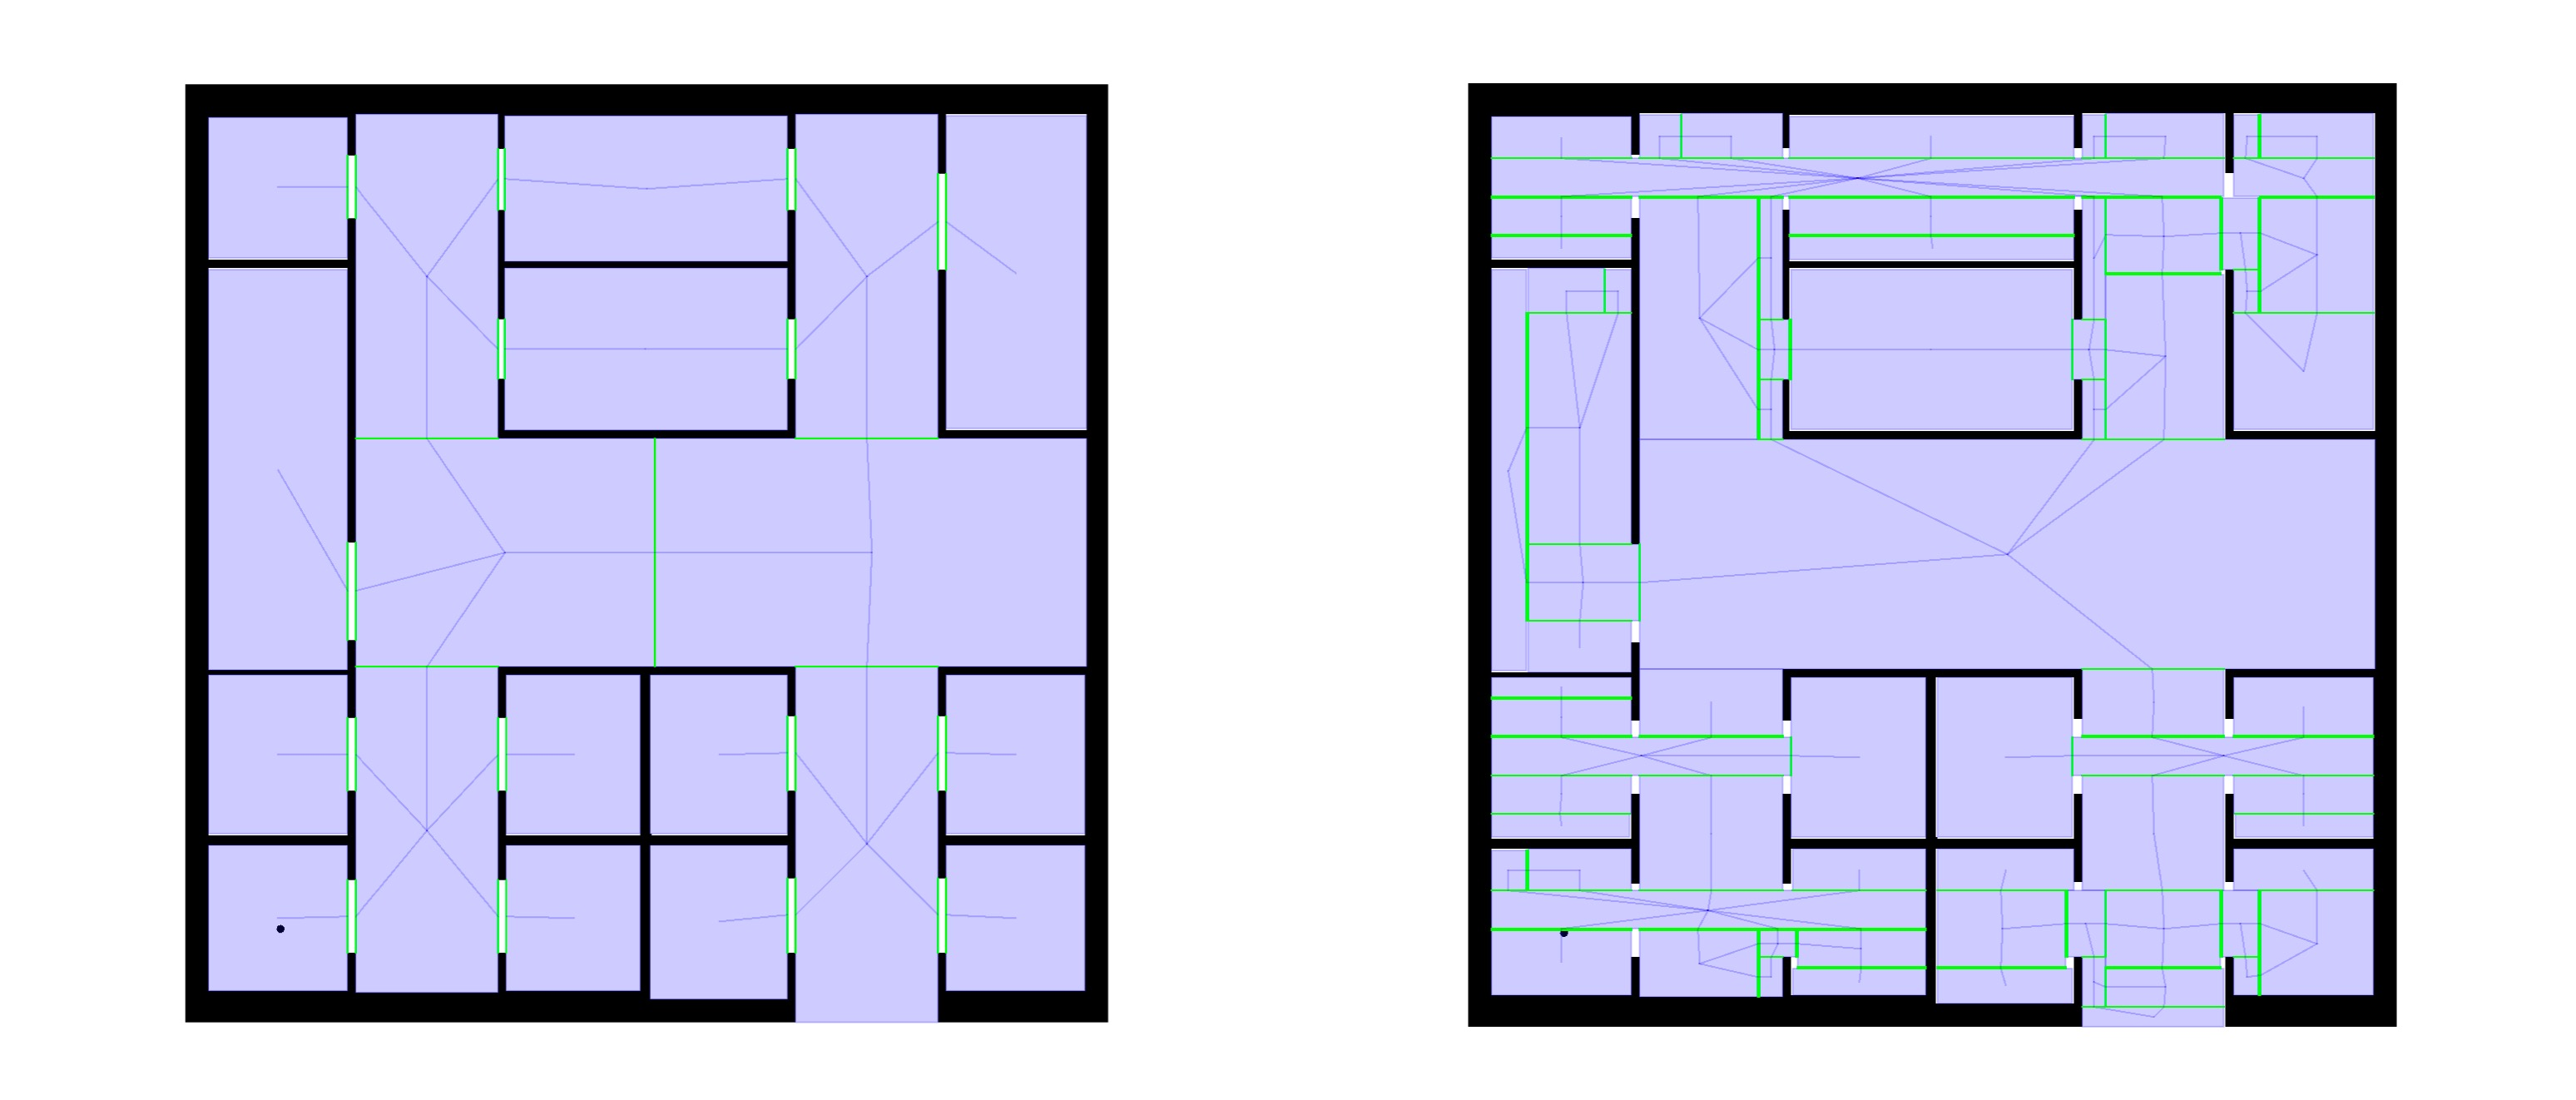
\includegraphics[width=\linewidth]{figures/envgraph.png}
	\caption{A sinistra: grafo dell'ambiente ottenuto in maniera semi automatica. A destra: grafo dell'ambiente ottenuto in maniera completamente automatica. I nodi sono poligoni convessi disegnati in blu, gli archi tra questi sono rappresentati con segmenti che congiungono il baricentro di ogni poligono al varco corrispondente. I varchi sono segmenti localizzati sui bordi dei poligoni convessi disegnati in verde.}
	\label{fig:envgraphs}
\end{figure}
\newline
Ottenere un grafo di navigazione soddisfacente può non essere triviale, nonostante il simulatore sia stato dotato di un algoritmo per la generazione di una tale struttura dati (come menzionato in fase di analisi), questo presenta diverse limitazioni ed è risultato inadeguato in più situazioni, rendendo necessario l'intervento umano per la generazione del grafo dell'ambiente. La direzione consigliata per gli sviluppi futuri inerenti questa problematica è la seguente: si dovranno modificare le abilità percettive dei pedoni in modo da renderle più realistiche; in particolare, facendo sì che questi possano percepire (e dunque valutare) solo i passaggi entro una certa distanza. Una tale tecnica è utile per ovviare al caso in cui i poligoni convessi generati fossero troppo grandi, ma è completamente inutile nel caso opposto. Pertanto, si ritiene indispensabile lo sviluppo di un algoritmo in grado di operare una buona divisione dell'ambiente in poligoni convessi in maniera completamente automatica. In particolare, una volta che le abilità percettive dei pedoni saranno ridimensionate i concetti di buona o cattiva divisione dell'ambiente assumeranno significati ben precisi: a parità (o quasi) di area coperta dai poligoni convessi generati, una divisione sarà tanto migliore quanto è minore il numero di poligoni.

I pedoni simulati in Alchemist sono al momento dotati di diverse caratteristiche psicologiche e sociali, e sono in grado di interagire sul piano psicologico. Sono invece assai limitate le caratteristiche fisiche e del tutto assenti le interazioni associate; il naturale corso di sviluppo porta alla realizzazione di pedoni dotati di vari aspetti fisici (e.g. stamina), di una forma realistica (ora sono modellati con semplici cerchi) e in grado di interagire tra loro sul piano fisico con spinte, urti e pressioni. Tali interazioni, in particolare, risultano estremamente importanti nonché interessanti al fine di introdurre nel simulatore aspetti come ferite o cadute; a tal proposito si veda quanto proposto in \cite{Pelechano2007}.

%----------------------------------------------------------------------------------------
% BIBLIOGRAPHY
%----------------------------------------------------------------------------------------

%\nocite{*} % uncomment this to show all the reference in the .bib file
\bibliographystyle{plain}
\bibliography{bibliography}

\appendix
\chapter{File di simulazione}

\section{Conoscenza completa dell'ambiente}
\lstinputlisting[
	%float,
	caption={File di simulazione del caso di studio presentato in \ref{complete-knowledge-case-study}}
]{listings/complete-knowledge.yml}

\section{Conoscenza parziale dell'ambiente}
\lstinputlisting[
	%float,
	caption={File di simulazione del caso di studio presentato in \ref{partial-knowledge-case-study}}
]{listings/partial-knowledge.yml}

\section{Nessuna conoscenza dell'ambiente}
\lstinputlisting[
	%float,
	caption={File di simulazione del caso di studio presentato in \ref{no-knowledge-case-study}}
]{listings/no-knowledge.yml}

\section{Evitare le congestioni}
\lstinputlisting[
	%float,
	caption={File di simulazione del caso di studio presentato in \ref{congestion-avoidance-case-study}}
]{listings/congestion-avoidance.yml}

\end{document}